%========================================================================================
%    PACKAGES AND THEMES
%========================================================================================

% This initializes a presentation document. aspectratio=169 makes the slides widescreen (16:9), which is standard for modern screens. xcolor=dvipsnames loads an extended palette of named colors (like "Green", "Maroon", etc.).
\documentclass[aspectratio=169,xcolor=dvipsnames]{beamer} 

% This applies a specific visual theme called "SimplePlus" to the slide
\usetheme{SimplePlus}

% Beamer has default boxes (blocks) you can put text inside. By default, an exampleblock is green but forces the title to be "Example". This custom code creates a new environment that keeps the nice green styling (bg=Green, bg=Green!10) but allows you to pass a custom title (#1) to the box.
\newenvironment{customexampleblock}[1]{%
% Title background color / foreground color
  \setbeamercolor{block title}{bg=Green, fg=white}

% Body background color / foreground color
  \setbeamercolor{block body}{bg=Green!10, fg=black} 
  \begin{block}{#1}
}{%
  \end{block}
}

\usepackage[utf8]{inputenc}
\usepackage[T1]{fontenc}
\usepackage[english]{babel}
\usepackage{amsmath, amssymb}
\usepackage{graphicx} % Allows including images
\usepackage{booktabs} % Allows the use of \toprule, \midrule and \bottomrule in tables
\usepackage{multirow}
\usepackage{hyperref}
\usepackage{caption} % Required for \captionof command
\usepackage{fontspec}

% This allows you to use system fonts rather than just standard LaTeX fonts. Specifically, it loads the Windows 11 "Segoe UI Emoji" font using the HarfBuzz text shaper.
\newfontface{\fluentemoji}{Segoe UI Emoji}[Renderer=HarfBuzz]

% This creates a shortcut command. If you type \emoji{🫀} in your document, it will render the actual color emoji perfectly on the slide.
\newcommand{\emoji}[1]{{\fluentemoji #1}}

%========================================================================================
%    TITLE PAGE
%========================================================================================

\title{Cost-Sensitive Learning for Myocardial Infarction Mortality Prediction: A Static and Dynamic Ensemble Framework}
\subtitle{} % No subtitle in the original, left empty
\author{Leonardo Saccotelli}
\institute{Università degli Studi di Bari Aldo Moro}
\date{} % Date left empty as in the original

\begin{document}

%========================================================================================
\section{Presentation Slides}
%========================================================================================

\begin{frame}
    % Print the title page as the first slide
    \titlepage
    
\end{frame}

%----------------------------------------------------------------------------------------

%\begin{frame}{Overview}
     % The \tableofcontents command will automatically list your sections and subsections
%     \tableofcontents
%\end{frame}

%========================================================================================
\section{Introduction and Motivations}
%========================================================================================

\begin{frame}

\frametitle{The Core Challenge in Clinical Prognosis}

    \begin{block}{Predicting Myocardial Infarction Outcome}
    	\begin{itemize}
            \item Early risk stratification of Myocardial Infarction (MI) at hospital admission is crucial for timely ICU resource allocation and patient survival.
            \item Clinical data inherently suffers from severe class imbalance.
            \item Standard ML algorithms naturally ignore the minority to maximize global accuracy.
        \end{itemize}  
	\end{block}
    
    \begin{block}{The Problem of Asymmetric Costs}
The real-world clinical cost of prediction errors is not equal:
        \begin{itemize}
            \item \textbf{False Positive (FP):} Predicting a lethal outcome for a survivor $\rightarrow$ A false alarm leading to over-triage (manageable resource cost).
            \item \textbf{False Negative (FN):} Predicting survival for a patient who ultimately dies $\rightarrow$ A missed intervention with \textbf{catastrophic consequences}.
        \end{itemize}
    \end{block}

\end{frame}

%----------------------------------------------------------------------------------------

\begin{frame}
\frametitle{Research Objectives \& Framework}

	\begin{block}{Primary Objective}
        To identify the most robust predictive pipeline for admission-time MI mortality by explicitly accounting for both minority-class rarity and asymmetric misclassification costs.
    \end{block}
    
    \begin{customexampleblock}{A Unified Experimental Comparison}
        We systematically evaluate models across two main dimensions:
        \begin{enumerate}
            \item \textbf{Model Architectures:} Linear baseline, \textit{Static Ensembles}, \textit{Dynamic Ensemble Selection} (DES) methods.
            \item \textbf{Cost-Sensitive Interventions:}
            \begin{itemize}
                \item \textbf{Learning-Level:} Data oversampling (SMOTE), class-frequency weighting, cost-matrix-driven weighting.
                \item \textbf{Decision-Level:} Standard 0.5 threshold, \textit{Minimum Expected Cost} (MEC) decision rule.
            \end{itemize}
        \end{enumerate}
    \end{customexampleblock}
    
\end{frame}

%========================================================================================
\section{Methodology}
%========================================================================================

\begin{frame}
\frametitle{Dataset Description and Construction}
            \begin{block}{Myocardial Infarction Complications Dataset \cite{golovenkin2020myocardial}}
                \begin{itemize}
\item \textbf{Source:} UCI Machine Learning Repository.
            \item \textbf{Scale:} 1700 records, 111 input features (demographics, ECG, medical history, labs).
            \item \textbf{Targets:} 12 variables (11 post-MI complications, 1 lethal outcome - \texttt{LET\_IS}).
            \item \textbf{Temporal Structure:} multiple ICU time points (admission, 24h, 48h, 72h).
                \end{itemize}
            \end{block}
    
            \begin{customexampleblock}{Time-Slice \& Target Formulation}
                \begin{itemize}
                    \item \textbf{Admission-Time Focus:} Retained only admission time for early prediction.
\item \textbf{Lethal Outcome Focus:} Retained only lethal outcome - \texttt{LET\_IS}.
                    \item \textbf{Binary Target Creation:} Collapsed the causes of death into a single positive class:
                    \begin{itemize}
                        \item \texttt{LET\_IS} $= 0 \rightarrow$ \textbf{0 (ALIVE)}
                        \item \texttt{LET\_IS} $\geq 1 \rightarrow$ \textbf{1 (DEAD)}
                    \end{itemize}
                \end{itemize}
            \end{customexampleblock}

\end{frame}

%----------------------------------------------------------------------------------------

\begin{frame}
\frametitle{Exploratory Data Analysis (EDA)}

	\begin{columns}[T]
    	\begin{column}{0.6\textwidth}
			\begin{block}{Insights from the Data}
				\begin{itemize}
                    \item \textbf{Data Quality:} Average missing rate 7.64\%,\\ 7 features >30\% missingness, 0 duplicates.
                    \item \textbf{Numerical Features:} Some show normal distributions, while several lab parameters are right-skewed with outliers. Strongest correlations are localized to blood pressure features.
                    \item \textbf{Categorical Features:} Several features are imbalanced, with frequencies concentrated in a few categories.
                    \item \textbf{Target Variable (\texttt{LET\_IS}):} Severely imbalanced, dominated by the \textbf{ALIVE (84.06\%)} class.
                \end{itemize}
            \end{block}
    	\end{column}

    	\begin{column}{0.4\textwidth}
        	\centering
        	
\includegraphics[width=\textwidth,height=3.75cm,keepaspectratio]{figures/correlation_matrix.png}
        	\vspace{0.3em}
        	\includegraphics[width=\textwidth,height=3.75cm,keepaspectratio]{figures/class_imbalance.png}
    	\end{column}
	\end{columns}
	
\end{frame}

%----------------------------------------------------------------------------------------

\begin{frame}
\frametitle{Data Cleaning \& Preprocessing}

    \begin{customexampleblock}{Missing Data Handling}
		\begin{itemize}
            \item \textbf{Filtering:} Records with >20\% missing values, features with >30\% missing values.
            \item \textbf{Imputation:} Median for numerical features, Mode for categorical features.
        \end{itemize}
    \end{customexampleblock}

    \begin{customexampleblock}{Type-Specific Feature Preprocessing}
        \begin{itemize}
            \item \textbf{Numerical Feature:} 
            \begin{itemize}
                \item Heavily right-skewed distribution $\rightarrow$ \texttt{log1p} + \texttt{StandardScaler}.
                \item Approximately normal distribution $\rightarrow$ \texttt{StandardScaler}.
            \end{itemize}
            
            \vspace{0.2em}
            
            \item \textbf{Categorical Feature:} 
            \begin{itemize}
                \item Nominal $\rightarrow$ \texttt{OneHotEncoder}.
                \item Binary $\rightarrow$ \texttt{LabelEncoder}.
                \item Ordinal $\rightarrow$ \texttt{OrdinalEncoder}.
            \end{itemize}
        \end{itemize}
    \end{customexampleblock}
\end{frame}

%----------------------------------------------------------------------------------------

\begin{frame}
\frametitle{Data Cleaning \& Preprocessing}   

	\begin{customexampleblock}{Custom Mapping (\texttt{ZSN\_A} - Chronic Heart Failure)}
        \begin{itemize}
            \item \textbf{Issue:} Partially ordered attribute with two intersecting severity lines ($0<1<2<4$ and $0<1<3<4$, where state 4 implies simultaneous states 2 and 3).
            \item \textbf{Solution:} Mapped into a 2D space to perfectly preserve severity structure:
            $$0 \rightarrow [0, 0] \quad 1 \rightarrow [1, 1] \quad 2 \rightarrow [2, 1] \quad 3 \rightarrow [1, 2] \quad 4 \rightarrow [3, 3]$$
        \end{itemize}
    \end{customexampleblock}
    
    \begin{customexampleblock}{Feature Selection}
		\begin{itemize}
            \item Applied \texttt{SelectKBest} using Mutual Information as the scoring criterion.
            \item The number of retained features ($k$) was embedded in the learning pipeline as a strictly tunable hyperparameter.
        \end{itemize}
    \end{customexampleblock}
    
\end{frame}

%----------------------------------------------------------------------------------------

\begin{frame}
\frametitle{Predictive Models: Logistic Regression}

    % ================= TOP SECTION: Two Columns =================
    \begin{columns}[c] % [c] vertically centers the content in the columns
        
        % LEFT COLUMN: Concept and Math
        \begin{column}{0.50\textwidth}
            \begin{block}{A Probabilistic Baseline}
            	A foundational linear model that serves as our highly interpretable baseline.
            	$$P(y=0 | \mathbf{x}) = \frac{1}{1 + exp(-\mathbf{w}^T \mathbf{x} - w_0)}$$
            \end{block}
        \end{column}
        
        % RIGHT COLUMN: Visual Representation
        \begin{column}{0.40\textwidth}
            \begin{center}
                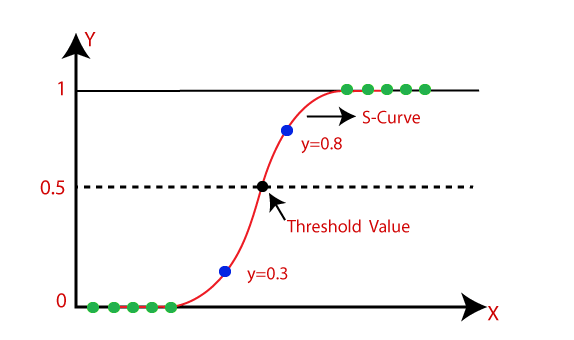
\includegraphics[width=\textwidth,keepaspectratio]{figures/sigmoid.png}
                \vspace{0.1em}
                \scriptsize \textit{The logistic curve maps raw scores to predicted probabilities.}
            \end{center}
        \end{column}
        
    \end{columns}

    \vspace{0.4em} % Adds breathing room between the top and bottom sections

    % ================= BOTTOM SECTION: Full Width =================
    \begin{customexampleblock}{Model Setup \& Hyperparameter Search Space}
        \begin{itemize}
            \item \texttt{solver: "liblinear"}, \texttt{penalty: "l2"}, \texttt{max\_iter:1000}
            \item \texttt{C} \(\in [10^{-4}, 10^{4})\), \texttt{tol} \(\in [10^{-5}, 10^{-2})\), \texttt{fit\_intercept} \(\in \{\texttt{True}, \texttt{False}\}\)

        \end{itemize}
    \end{customexampleblock}

\end{frame}

%----------------------------------------------------------------------------------------

\begin{frame}
\frametitle{Predictive Models: Random Forest}

    % ================= TOP SECTION: Two Columns =================
    \begin{columns}[c] % [c] vertically centers the content in the columns
        
        % LEFT COLUMN: Concept and Math
        \begin{column}{0.60\textwidth}
            \begin{block}{Static Ensembles -- Bagging Paradigm}
            An ensemble learning method that builds multiple decorrelated decision trees by learning them on a:
            	\begin{itemize}
            		\item randomly chosen subset of input variables,
            		\item randomly chosen subset of data samples.
		    	\end{itemize}
            \end{block}
        \end{column}
        
        % RIGHT COLUMN: Visual Representation
        \begin{column}{0.35\textwidth}
            \begin{center}
                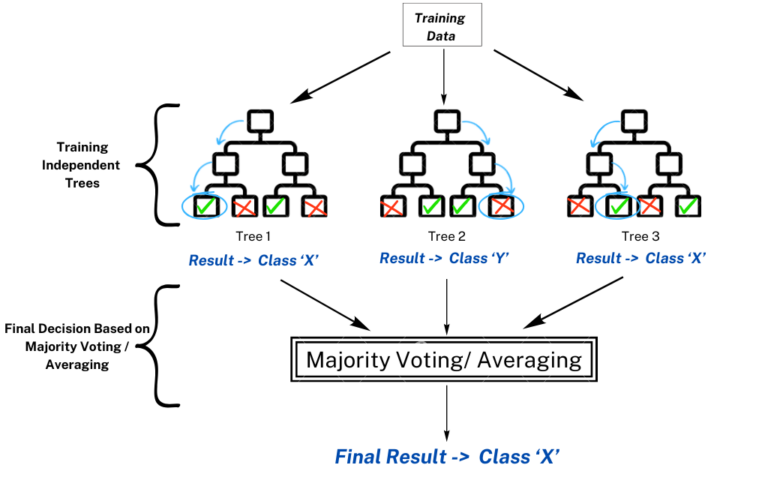
\includegraphics[width=\textwidth,keepaspectratio]{figures/rf.png}
            \end{center}
        \end{column}
        
    \end{columns}

    \vspace{0.1em} % Adds breathing room between the top and bottom sections

    % ================= BOTTOM SECTION: Full Width =================
    \begin{customexampleblock}{Model Setup \& Hyperparameter Search Space}
        \begin{itemize}
            \item \texttt{criterion: "gini"}, \texttt{bootstrap: "True"}
            \item \texttt{n\_estimators} \(\in [100, 1000)\), \texttt{max\_samples} \(\in [0.5, 0.9)\), \texttt{max\_depth} \(\in [3, 20)\),
\texttt{max\_features} \(\in \{\texttt{sqrt}, \texttt{log2}, \texttt{None}\}\),
 \texttt{min\_samples\_split} \(\in [2, 10)\), \texttt{min\_samples\_leaf} \(\in [1, 10)\), \texttt{max\_leaf\_nodes} \(\in [2, 20)\), \texttt{ccp\_alpha} \(\in [0.0, 0.01)\) \texttt{min\_impurity\_decrease} \(\in [0.0, 0.1)\)

        \end{itemize}
    \end{customexampleblock}

\end{frame}

%----------------------------------------------------------------------------------------

\begin{frame}
\frametitle{Predictive Models: XGBoost}

    % ================= TOP SECTION: Two Columns =================
    \begin{columns}[c]
        
        % LEFT COLUMN: Concept and Math
        \begin{column}{0.55\textwidth}
            \begin{block}{Static Ensembles -- Boosting Paradigm}
                XGBoost is an optimized gradient boosting algorithm that combines multiple decision trees as base learners, building them sequentially:
                \begin{itemize}
            		\item each tree corrects errors of the previous one,
            		\item sum the predictions of all the trees.
		    	\end{itemize}

            \end{block}
        \end{column}
        
        % RIGHT COLUMN: Visual Representation
        \begin{column}{0.42\textwidth}
            \begin{center}
                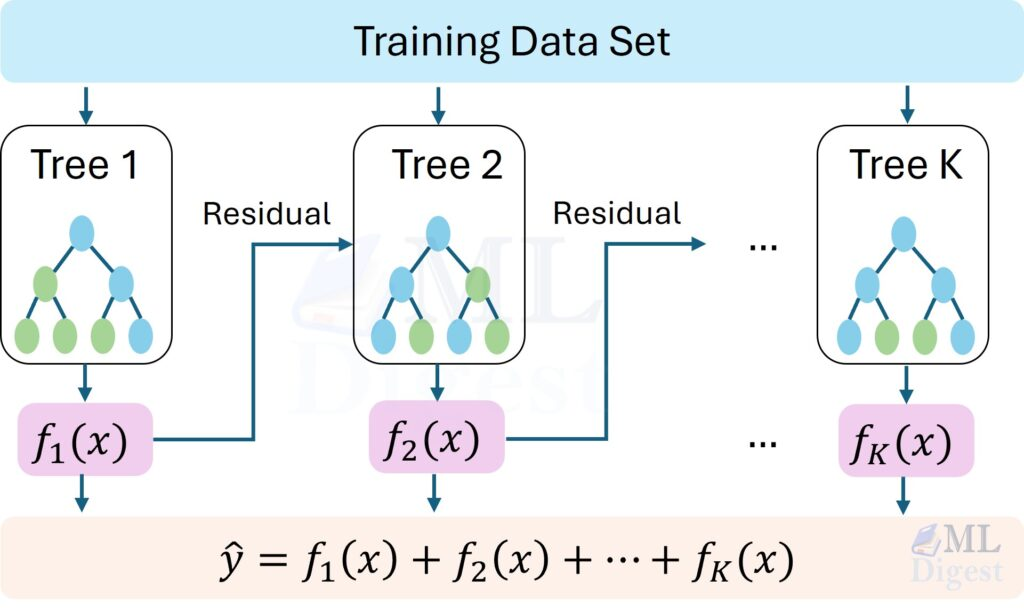
\includegraphics[width=\textwidth,keepaspectratio]{figures/xgboost.png}
            \end{center}
        \end{column}
        
    \end{columns}

    \vspace{1em}

    % ================= BOTTOM SECTION: Full Width =================
    \begin{customexampleblock}{Model Setup \& Hyperparameter Search Space}
        \begin{itemize}
            \item \texttt{objective: "binary:logistic"}, \texttt{eval\_metric: "logloss"}
            \item \texttt{n\_estimators} \(\in [200, 800)\), \texttt{learning\_rate} \(\in [10^{-2}, 0.2)\), \texttt{max\_depth} \(\in [3, 10)\), \texttt{subsample} \(\in [0.6, 1.0)\), \texttt{colsample\_bytree} \(\in [0.6, 1.0)\), \texttt{gamma} \(\in [0.0, 5.0)\), \texttt{reg\_alpha} \(\in [10^{-4}, 10)\), \texttt{reg\_lambda} \(\in [10^{-4}, 10)\), \texttt{min\_child\_weight} \(\in [1, 10)\)

        \end{itemize}
    \end{customexampleblock}

\end{frame}

%----------------------------------------------------------------------------------------

\begin{frame}
\frametitle{Predictive Models: Voting}

	\begin{columns}[T]
    	\begin{column}{0.63\textwidth}
    		\begin{block}{Static Ensembles -- Voting Paradigm}
				\begin{itemize}
					\item \textbf{Heterogeneous Pool:} Random Forest, XGBoost, and SGD Classifier (\texttt{loss="log\_loss"}, \texttt{alpha} \(\in [10^{-5}, 10)\), \texttt{l1\_ratio} \(\in [0, 1)\), \texttt{penalty} \(\in \{\texttt{l2}, \texttt{l1}, \texttt{elasticnet}\}\)).
					\item \textbf{Independent Tuning:} Each base learner is independently optimized.
					\item \textbf{Soft Voting :} Gathers the predicted probabilities from all base models and computes the simple mathematical average (uniform weights) to output a robust final decision.
        		\end{itemize}
			\end{block}
    	\end{column}

    	\begin{column}{0.37\textwidth}
    		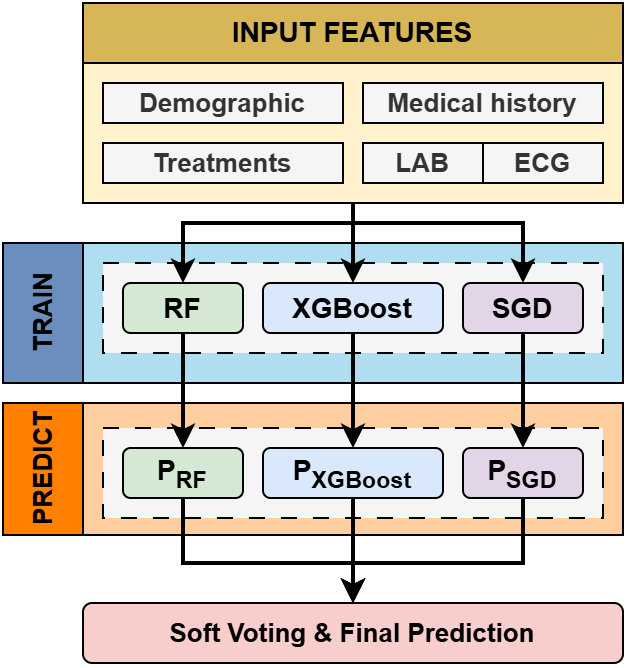
\includegraphics[width=\textwidth,keepaspectratio]{figures/voting.png}
    	\end{column}
	\end{columns}

\end{frame}

%----------------------------------------------------------------------------------------

\begin{frame}
\frametitle{Predictive Models: Stacking}
	\begin{block}{Static Ensembles -- Stacking Paradigm}
		\begin{itemize}
			\item \textbf{Heterogeneous Pool:} Random Forest, XGBoost, and SGD Classifier.
			\item \textbf{Independent Tuning:} Each base learner is independently optimized.
			\item \textbf{Cross-Validated Inputs:} The base learners generate out-of-fold predictions using a \texttt{cv=3} splitting strategy to prevent overfitting.                    
            \item \textbf{Meta-Estimator:} These intermediate predictions become the \textit{new input features} for a higher-level algorithm (\texttt{LogisticRegression}).
       	\end{itemize}
	\end{block}

	\begin{center}
		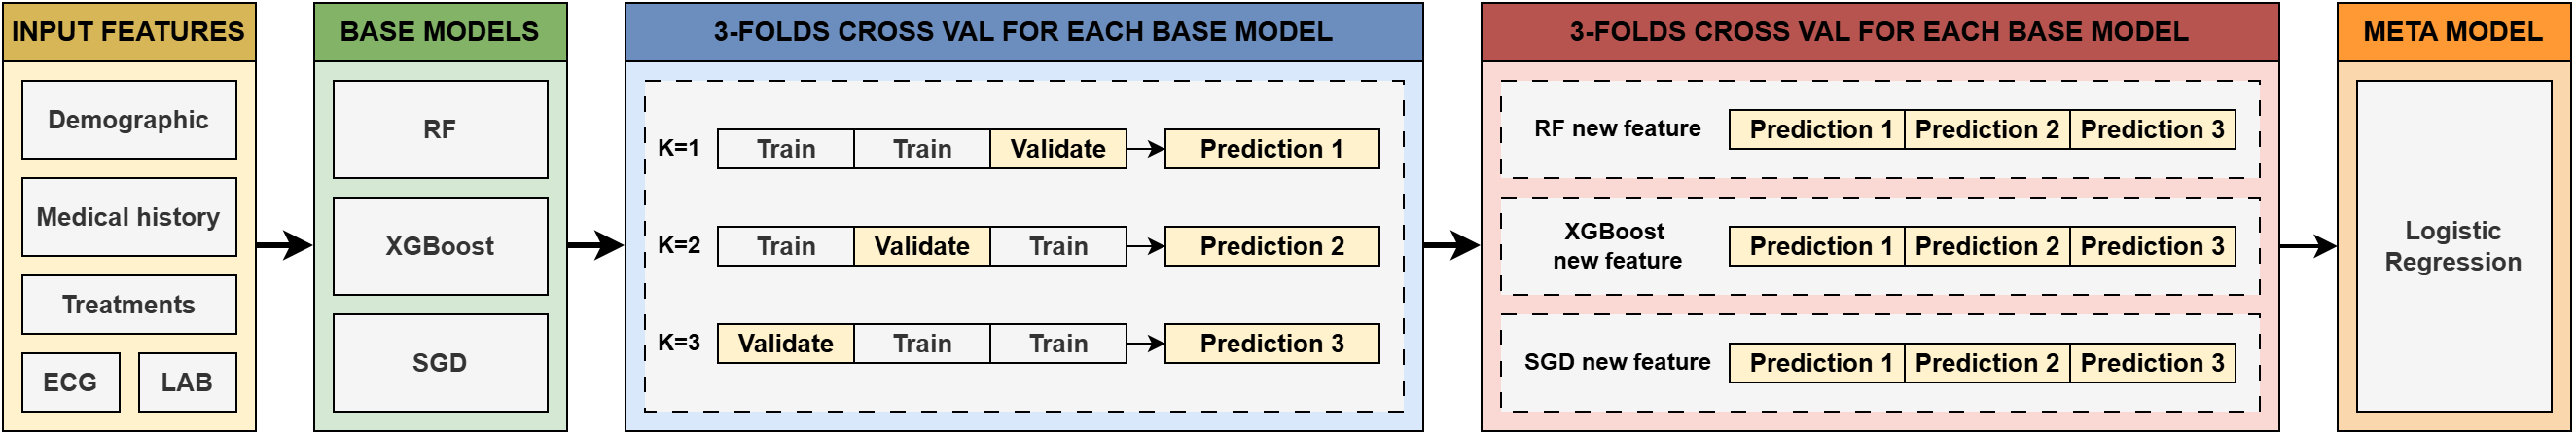
\includegraphics[width=\textwidth,height=0.75\textheight,keepaspectratio]{figures/stacking.png}
    \end{center}

\end{frame}

%----------------------------------------------------------------------------------------

\begin{frame}
\frametitle{Predictive Models: Dynamic Ensemble Selection}

	\begin{block}{The Dynamic Paradigm \cite{CRUZ2018195}}
		Unlike static models that rely on a fixed ensemble for all instances, DES selects the most competent subset of classifiers $C' \subseteq C$ for \textit{each specific query sample $x_j$} based on its local context. The selected ensemble $C'$ is finally integrated to produce the decision for $x_j$.

	\end{block}
	
	\vspace{1em}
	\begin{center}		
		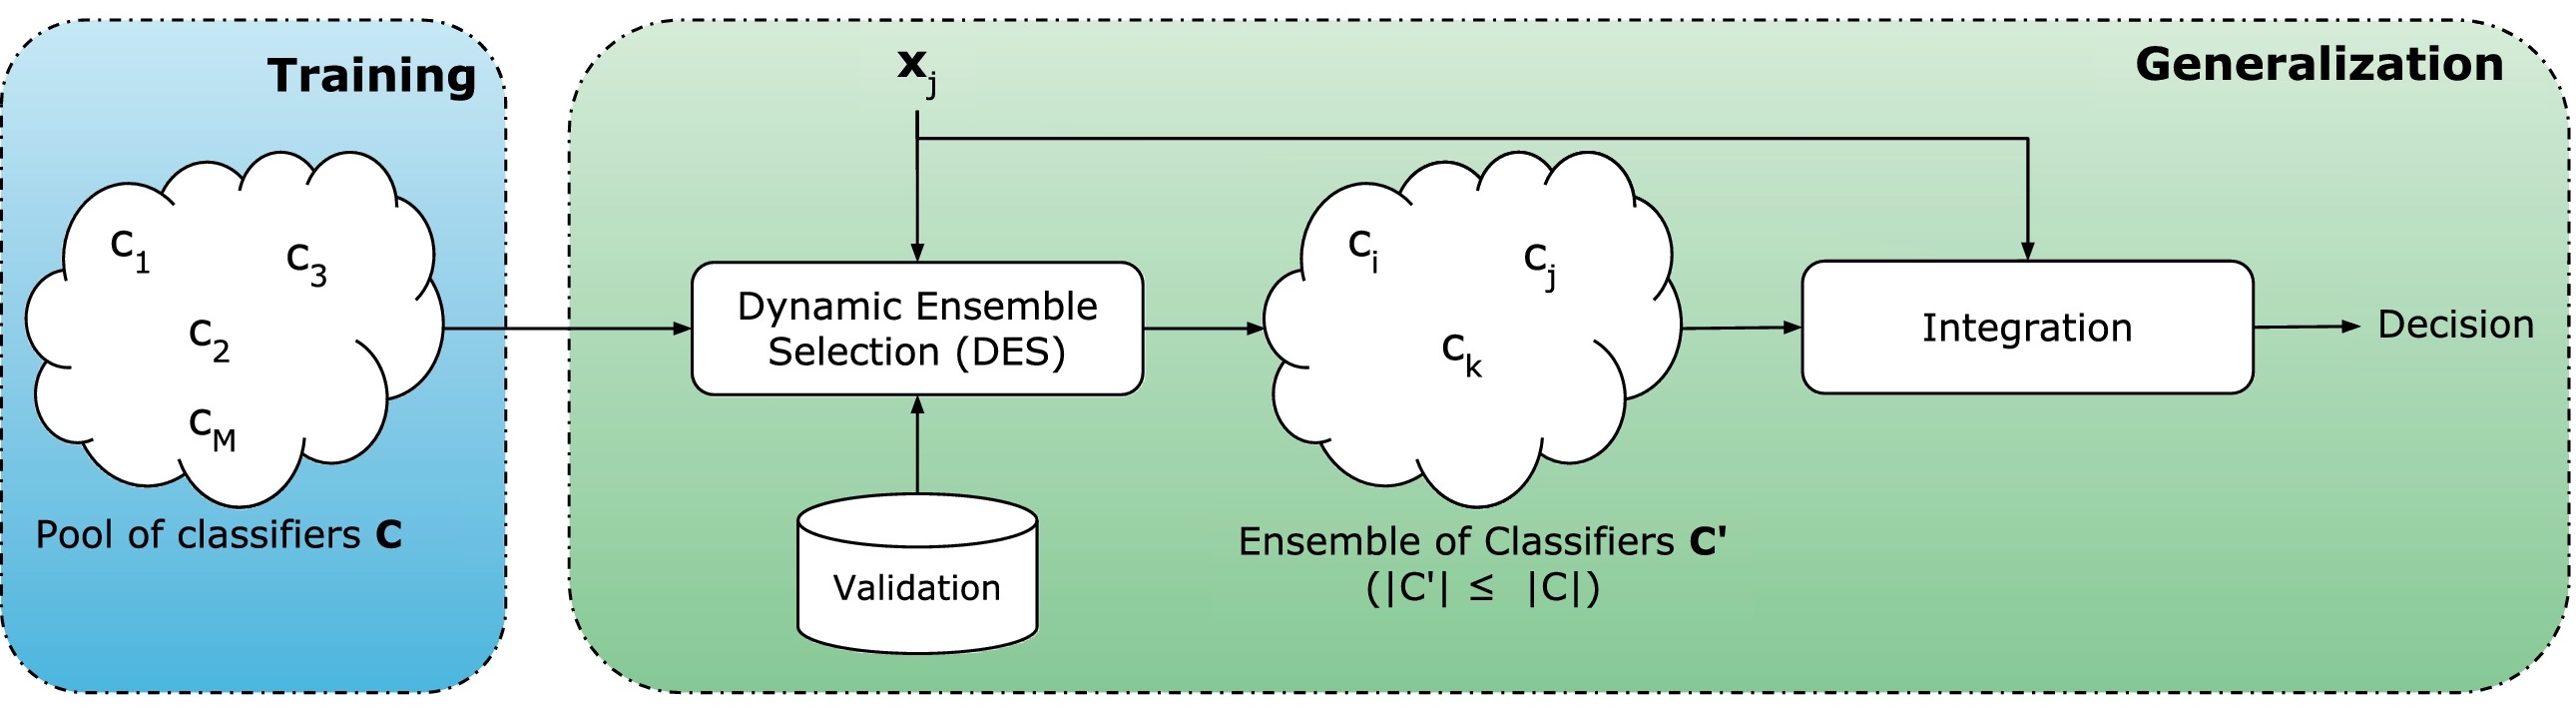
\includegraphics[width=0.95\textwidth,height=0.4\textheight,keepaspectratio]{figures/des2.png}
	\end{center}

\end{frame}

%----------------------------------------------------------------------------------------

\begin{frame}
\frametitle{Predictive Models: Dynamic Ensemble Selection}
	\begin{block}{The 3-Phase Architecture}
		\begin{enumerate}
			\item \textbf{Generation:} A diverse pool of classifiers is built.
			\item \textbf{Selection:} For a new query, a local "region of competence" is defined using a dedicated dataset (\textbf{DSEL}). The system evaluates and selects the local experts.
			\item \textbf{Integration:} The predictions of the dynamically selected subset are aggregated to form the final decision.
        	\end{enumerate}
	\end{block}
	
	\vspace{1em}
	\begin{center}		
		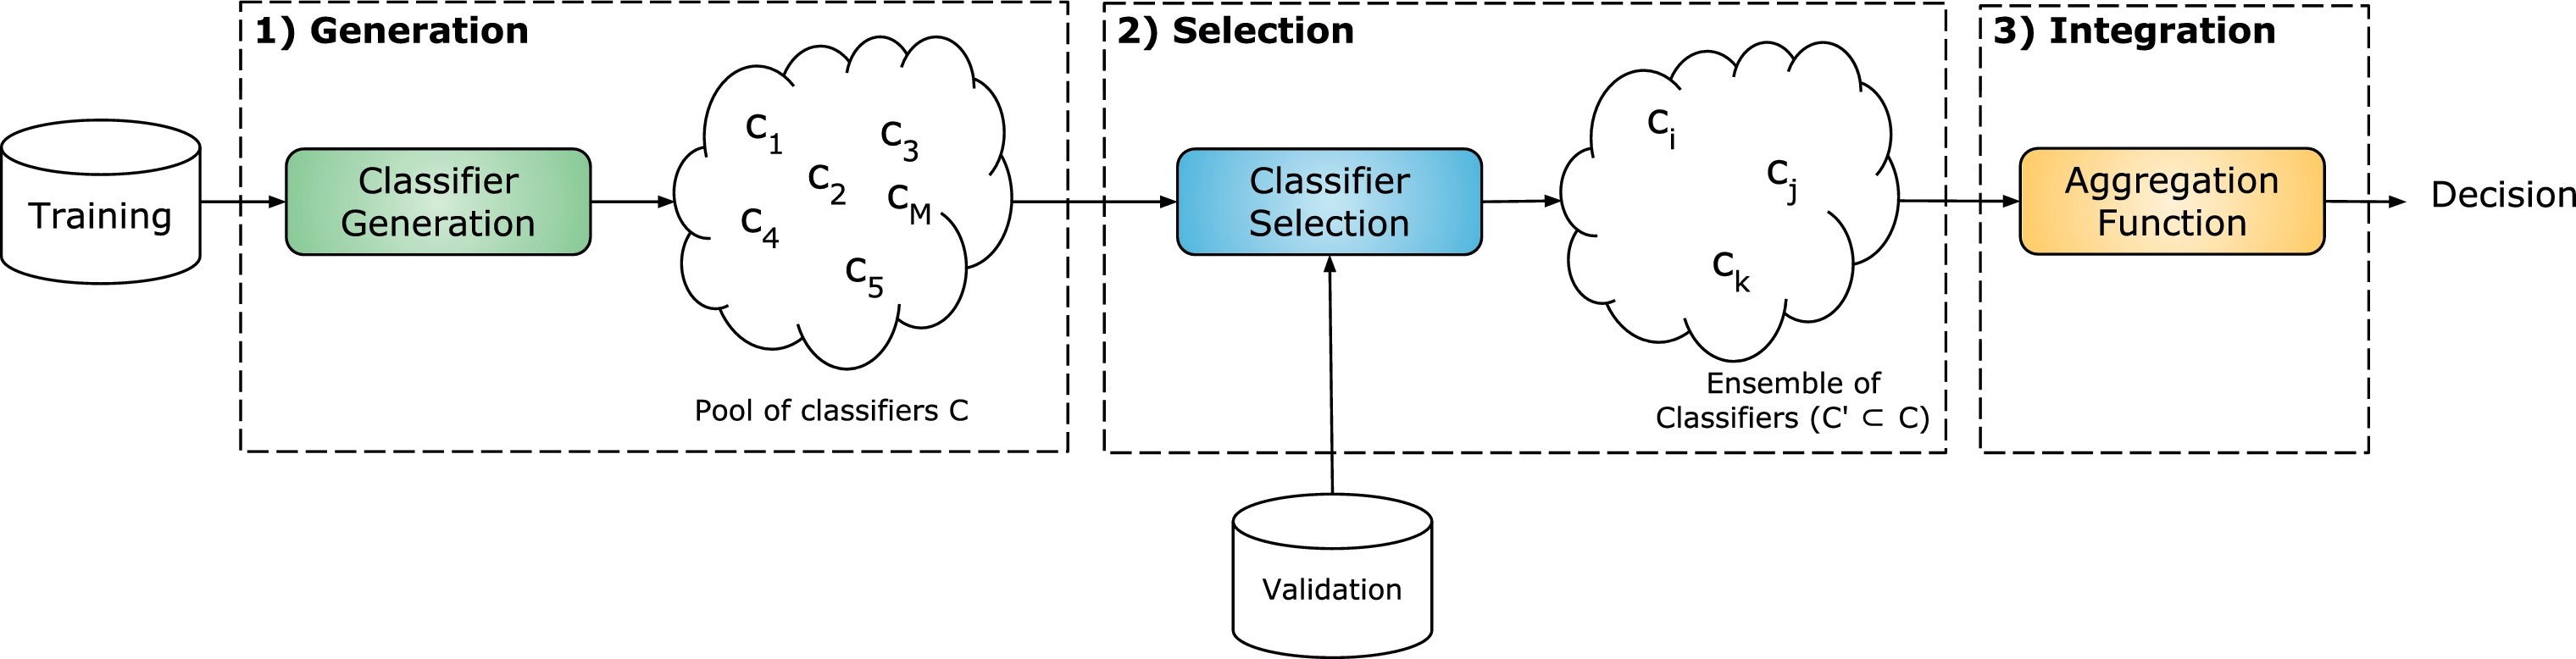
\includegraphics[width=0.95\textwidth,height=0.4\textheight,keepaspectratio]{figures/des1.png}
	\end{center}

\end{frame}

%----------------------------------------------------------------------------------------

\begin{frame}
\frametitle{Predictive Models: Dynamic Ensemble Selection}

\begin{block}{1. KNORA-E (Oracle-Based)}
        \begin{itemize}
            \item Identifies local "experts" that \textit{perfectly} classify all samples in the query's defined region of competence.
            \item Dynamically shrinks the neighborhood size (removes the furthest neighbor) if no perfect oracle is initially found.
        \end{itemize}
    \end{block}

    \begin{block}{2. DES-KL (Information Theory)}
        \begin{itemize}
            \item Evaluates competence via a distance-weighted Gaussian potential function within the local k-NN neighborhood.
            \item Computes the Kullback--Leibler (KL) divergence between a base classifier's output profile and a Random Classifier. Models performing significantly better than random guessing are selected.
        \end{itemize}
    \end{block}

\end{frame}

%----------------------------------------------------------------------------------------

\begin{frame}
\frametitle{Predictive Models: Dynamic Ensemble Selection}

\begin{block}{3. META-DES (Meta-Learning)}
        \begin{itemize}
            \item Extracts advanced local meta-features (e.g., neighborhood consensus, model confidence) for each query.
            \item Utilizes a trained Multinomial Naive Bayes meta-classifier to explicitly predict if a base-learner is competent enough to be selected.
        \end{itemize}
    \end{block}

\begin{customexampleblock}{Implementation Specifics}
        \begin{itemize}
            \item \textbf{Base Classifier Pool:} \texttt{BaggingClassifier} of \texttt{DecisionTreeClassifier}
            \begin{itemize}
            	\item \texttt{n\_estimators} \(\in [100, 1000)\), \texttt{max\_samples} \(\in [0.5, 0.9)\),
            \texttt{max\_depth} \(\in [3, 20)\), \texttt{min\_samples\_split} \(\in [2, 10)\), \texttt{min\_samples\_leaf} \(\in [1, 10)\), \texttt{ccp\_alpha} \(\in [0.0, 0.01)\), \texttt{max\_leaf\_nodes} \(\in [2, 20)\), \texttt{min\_impurity\_decrease} \(\in [0.0, 0.1)\).
                
			\end{itemize}             
                                    
            \item \textbf{Region of Competence:} Computed using the $k$-Nearest Neighbors ($K=7$).
                       
        \end{itemize}
    \end{customexampleblock}

\end{frame}

%----------------------------------------------------------------------------------------

\begin{frame}
\frametitle{Imbalance-Aware: Learning-Level Strategies}

    \begin{block}{Data-Level Strategy: SMOTE \cite{Araf2024}}
\begin{itemize}
            \item \textbf{Objective:} Synthetically oversamples the minority class within the training set.
            \item \textbf{Mechanism:} Locates the $k$-nearest neighbors ($k=5$) for a minority sample and interpolates a new synthetic instance along the connecting line.
            \item \textbf{Outcome:} Achieves a balanced class distribution prior to model training according to a defined oversampling ratio.
        \end{itemize}
    \end{block}
    
    \vspace{0.5em}
    \centering
    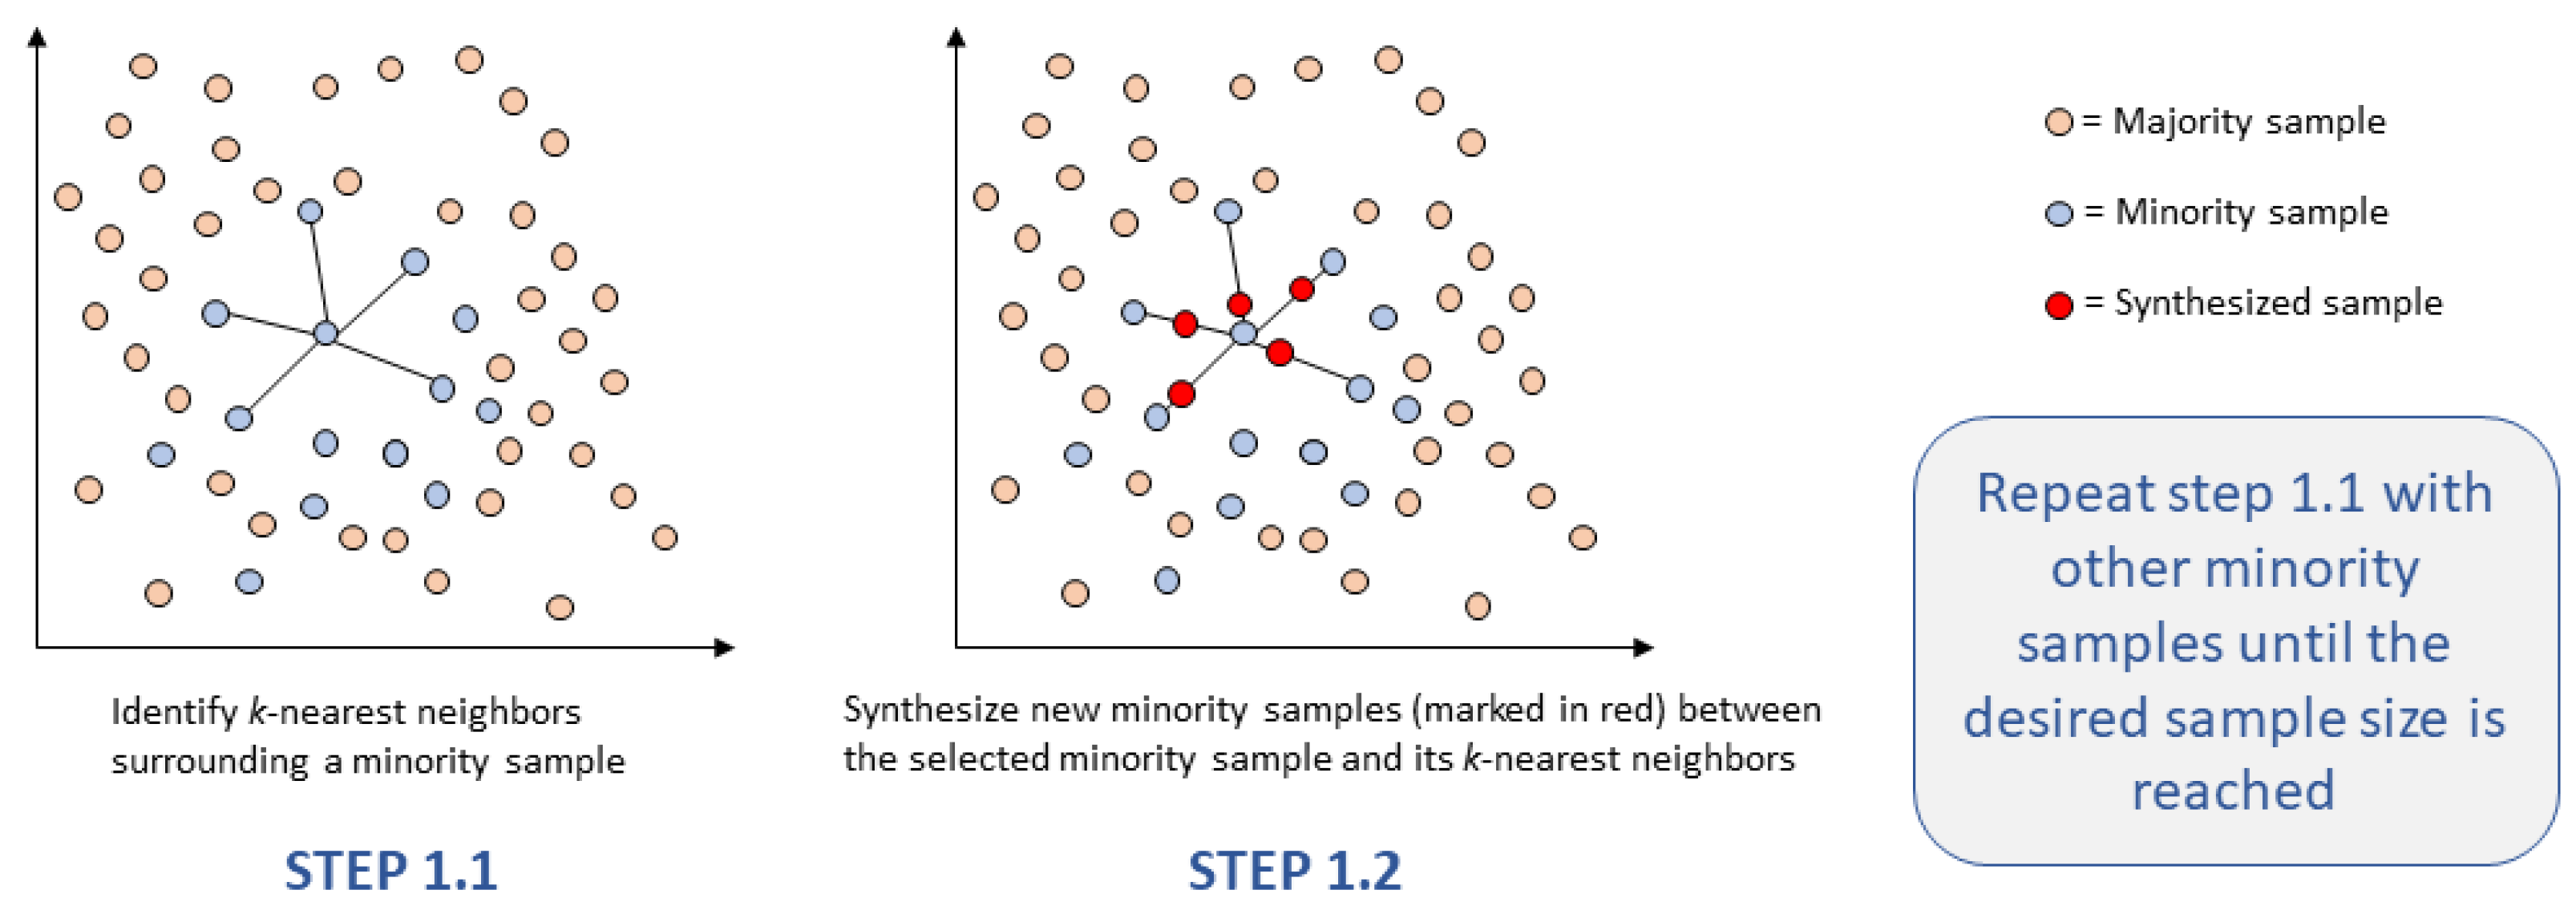
\includegraphics[width=\textwidth,height=3.75cm,keepaspectratio]{figures/SMOTE.png}

\end{frame}

%----------------------------------------------------------------------------------------

\begin{frame}
\frametitle{Imbalance-Aware: Learning-Level Strategies}

\begin{block}{Algorithm-Level Strategy: Class-Frequency Weighting \cite{Araf2024}}
        \begin{itemize}
            \item \textbf{Objective:} Penalize misclassifications of the minority class by assigning higher weights directly inside the algorithm's loss function.
            \item \textbf{Mechanism:} Weights are automatically derived from the inverse of the class frequencies in the training data.
        \end{itemize}
    \end{block}
    
    \vspace{0.2cm}
    
    \begin{customexampleblock}{Implementation Frameworks}
        \begin{itemize}
            \item \textbf{Scikit-Learn Library (\texttt{class\_weight="balanced"}):} 
            \begin{itemize}
                \item Computes weights inversely proportional to class frequencies.
                \item \texttt{class\_weight = \{0:} $\frac{n_{\text{samples}}}{2 \cdot n_0}$\texttt{, 1:} $\frac{n_{\text{samples}}}{2 \cdot n_1}$\texttt{\}}
            \end{itemize}
            
            \vspace{0.1cm}
            
            \item \textbf{XGBoost Library (\texttt{scale\_pos\_weight}):} 
            \begin{itemize}
                \item Used in XGBoost to scale the gradient of the positive class.
                \item Calculated as the ratio of negative to positive samples: $\frac{n_0}{n_1}$
            \end{itemize}
        \end{itemize}
    \end{customexampleblock}

\end{frame}

%----------------------------------------------------------------------------------------

\begin{frame}
\frametitle{Imbalance-Aware: Learning-Level Strategies}

\begin{block}{Algorithm-Level Strategy: Cost-Sensitive Learning \cite{Araf2024}}
        \begin{itemize}
            \item \textbf{Objective:} Explicitly guide the loss function during training using predefined, asymmetric clinical costs rather than dataset frequencies.
        \end{itemize}
    \end{block}
    
    \vspace{0.1cm}
                
    \begin{customexampleblock}{The Clinical Cost Matrix}
        \vspace{0.1cm}

		\centering
		\begin{tabular}{l c c}
		\toprule
		& \textbf{Predicted: ALIVE (0)} & \textbf{Predicted: DEAD (1)} \\
		\midrule
		\textbf{Actual: ALIVE (0)} & TN=0 & FP=1 \\
		\textbf{Actual: DEAD (1)} & \textcolor{red}{\textbf{FN=10}} & TP=0 \\
		\bottomrule
	\end{tabular}
        
        \vspace{0.2cm}
        A missed lethal outcome (FN) is penalized \textbf{10x} more heavily than a false alarm (FP).
        
        \begin{itemize}
    		\item \textbf{Implementation:} \texttt{class\_weight=\{0:1, \textcolor{red}{\textbf{1:10}}\}} or \texttt{scale\_pos\_weight=\textcolor{red}{\textbf{10}}}.
    	\end{itemize}
    \end{customexampleblock}
\end{frame}

%----------------------------------------------------------------------------------------

\begin{frame}
\frametitle{Imbalance-Aware: Decision-Level Strategies}

    \begin{block}{1. Standard Threshold}
    	\begin{itemize}
    		\item Standard ML models use a default threshold of 0.5 to assign classes.
    		\item A 0.5 threshold implicitly assumes that FP and FN have equal clinical cost.
    	\end{itemize}
    \end{block}
    
    \begin{block}{2. Minimum Expected Cost (MEC) \cite{elkan2001}}
    	\begin{itemize}
    		\item MEC computes the optimal threshold based on the misclassification cost.
    		\item MEC selects the class that minimizes the expected misclassification cost.
    	\end{itemize}
    	
    	        $$ \hat{y} = \arg\min_{c} \sum_{k} P(y=k \mid x)\, C_{k,c} $$
        
        \begin{itemize}
            \item $P(y=k \mid x)$ = Predicted posterior probability.
            \item $C_{k,c}$ = The specific cost from the matrix (e.g., \textcolor{red}{\textbf{FN=10}}, FP=1).
            \item \textbf{Result:} Model predictions are strictly aligned with real-world clinical cost.
        \end{itemize}
    \end{block}
   
\end{frame}

%========================================================================================
\section{Experiment Setup}
%========================================================================================
\begin{frame}
\frametitle{Imbalance-Aware: Experimental Settings}
	We systematically compared \textbf{7} configurations: \textbf{1 standard baseline}, \textbf{6 imbalance-aware}.

    \vspace{0.3em}
    \begin{customexampleblock}{Systematic Configuration Grid}
        \centering
        \small
        \renewcommand{\arraystretch}{1.3} % Adds a bit of vertical breathing room
        \begin{tabular}{@{} l l c l @{}}
            \toprule
            \textbf{Imbalance Strategy (Learning)} & \textbf{Decision Threshold} & & \textbf{Experiment Alias} \\
            \midrule            
            
            % Baseline
            None (Cost-Insensitive) & Standard (0.5) & $\rightarrow$ & \texttt{Baseline} \\
                        
            % Balanced
            Class-Frequency Weighting & Standard (0.5) & $\rightarrow$ & \texttt{Balanced + STD} \\
            Class-Frequency Weighting & MEC Policy & $\rightarrow$ & \texttt{Balanced + MEC} \\
            
            % Cost-sensitive
            Cost-Matrix Weighting (\textcolor{red}{\textbf{1:10}}) & Standard (0.5) & $\rightarrow$ & \texttt{Cost-sensitive + STD} \\
            Cost-Matrix Weighting (\textcolor{red}{\textbf{1:10}}) & MEC Policy & $\rightarrow$ & \texttt{Cost-sensitive + MEC} \\
            
            % SMOTE
            SMOTE (Data Oversampling) & Standard (0.5) & $\rightarrow$ & \texttt{SMOTE + STD} \\
            SMOTE (Data Oversampling) & MEC Policy & $\rightarrow$ & \texttt{SMOTE + MEC} \\
            
            \bottomrule
        \end{tabular}
        \vspace{0.5em}
    \end{customexampleblock}   

\end{frame}

%----------------------------------------------------------------------------------------

\begin{frame}
\frametitle{Learning Pipeline: Logistic Regression \& Static Ensembles}

    % ================= TOP SECTION: Two Columns =================
    \begin{columns} % [c] vertically centers the content in the columns
        
        % LEFT COLUMN: Concept and Math
        \begin{column}{0.35\textwidth}
    		\begin{customexampleblock}{Evaluation Protocol}
        		\begin{itemize}
            			\item \textbf{Evaluation (Outer Loop):} Repeated Stratified 10$\times$10 CV.
            			\item \textbf{Tuning (Inner Loop):} Stratified 5-Fold CV.
            			\item \textbf{Tuning Algorithm:} \texttt{Random Search} (\texttt{n\_iter=30}).
        		\end{itemize}
            \end{customexampleblock}
            
        \end{column}
        
        % RIGHT COLUMN: Visual Representation
        \begin{column}{0.60\textwidth}
		\centering
   		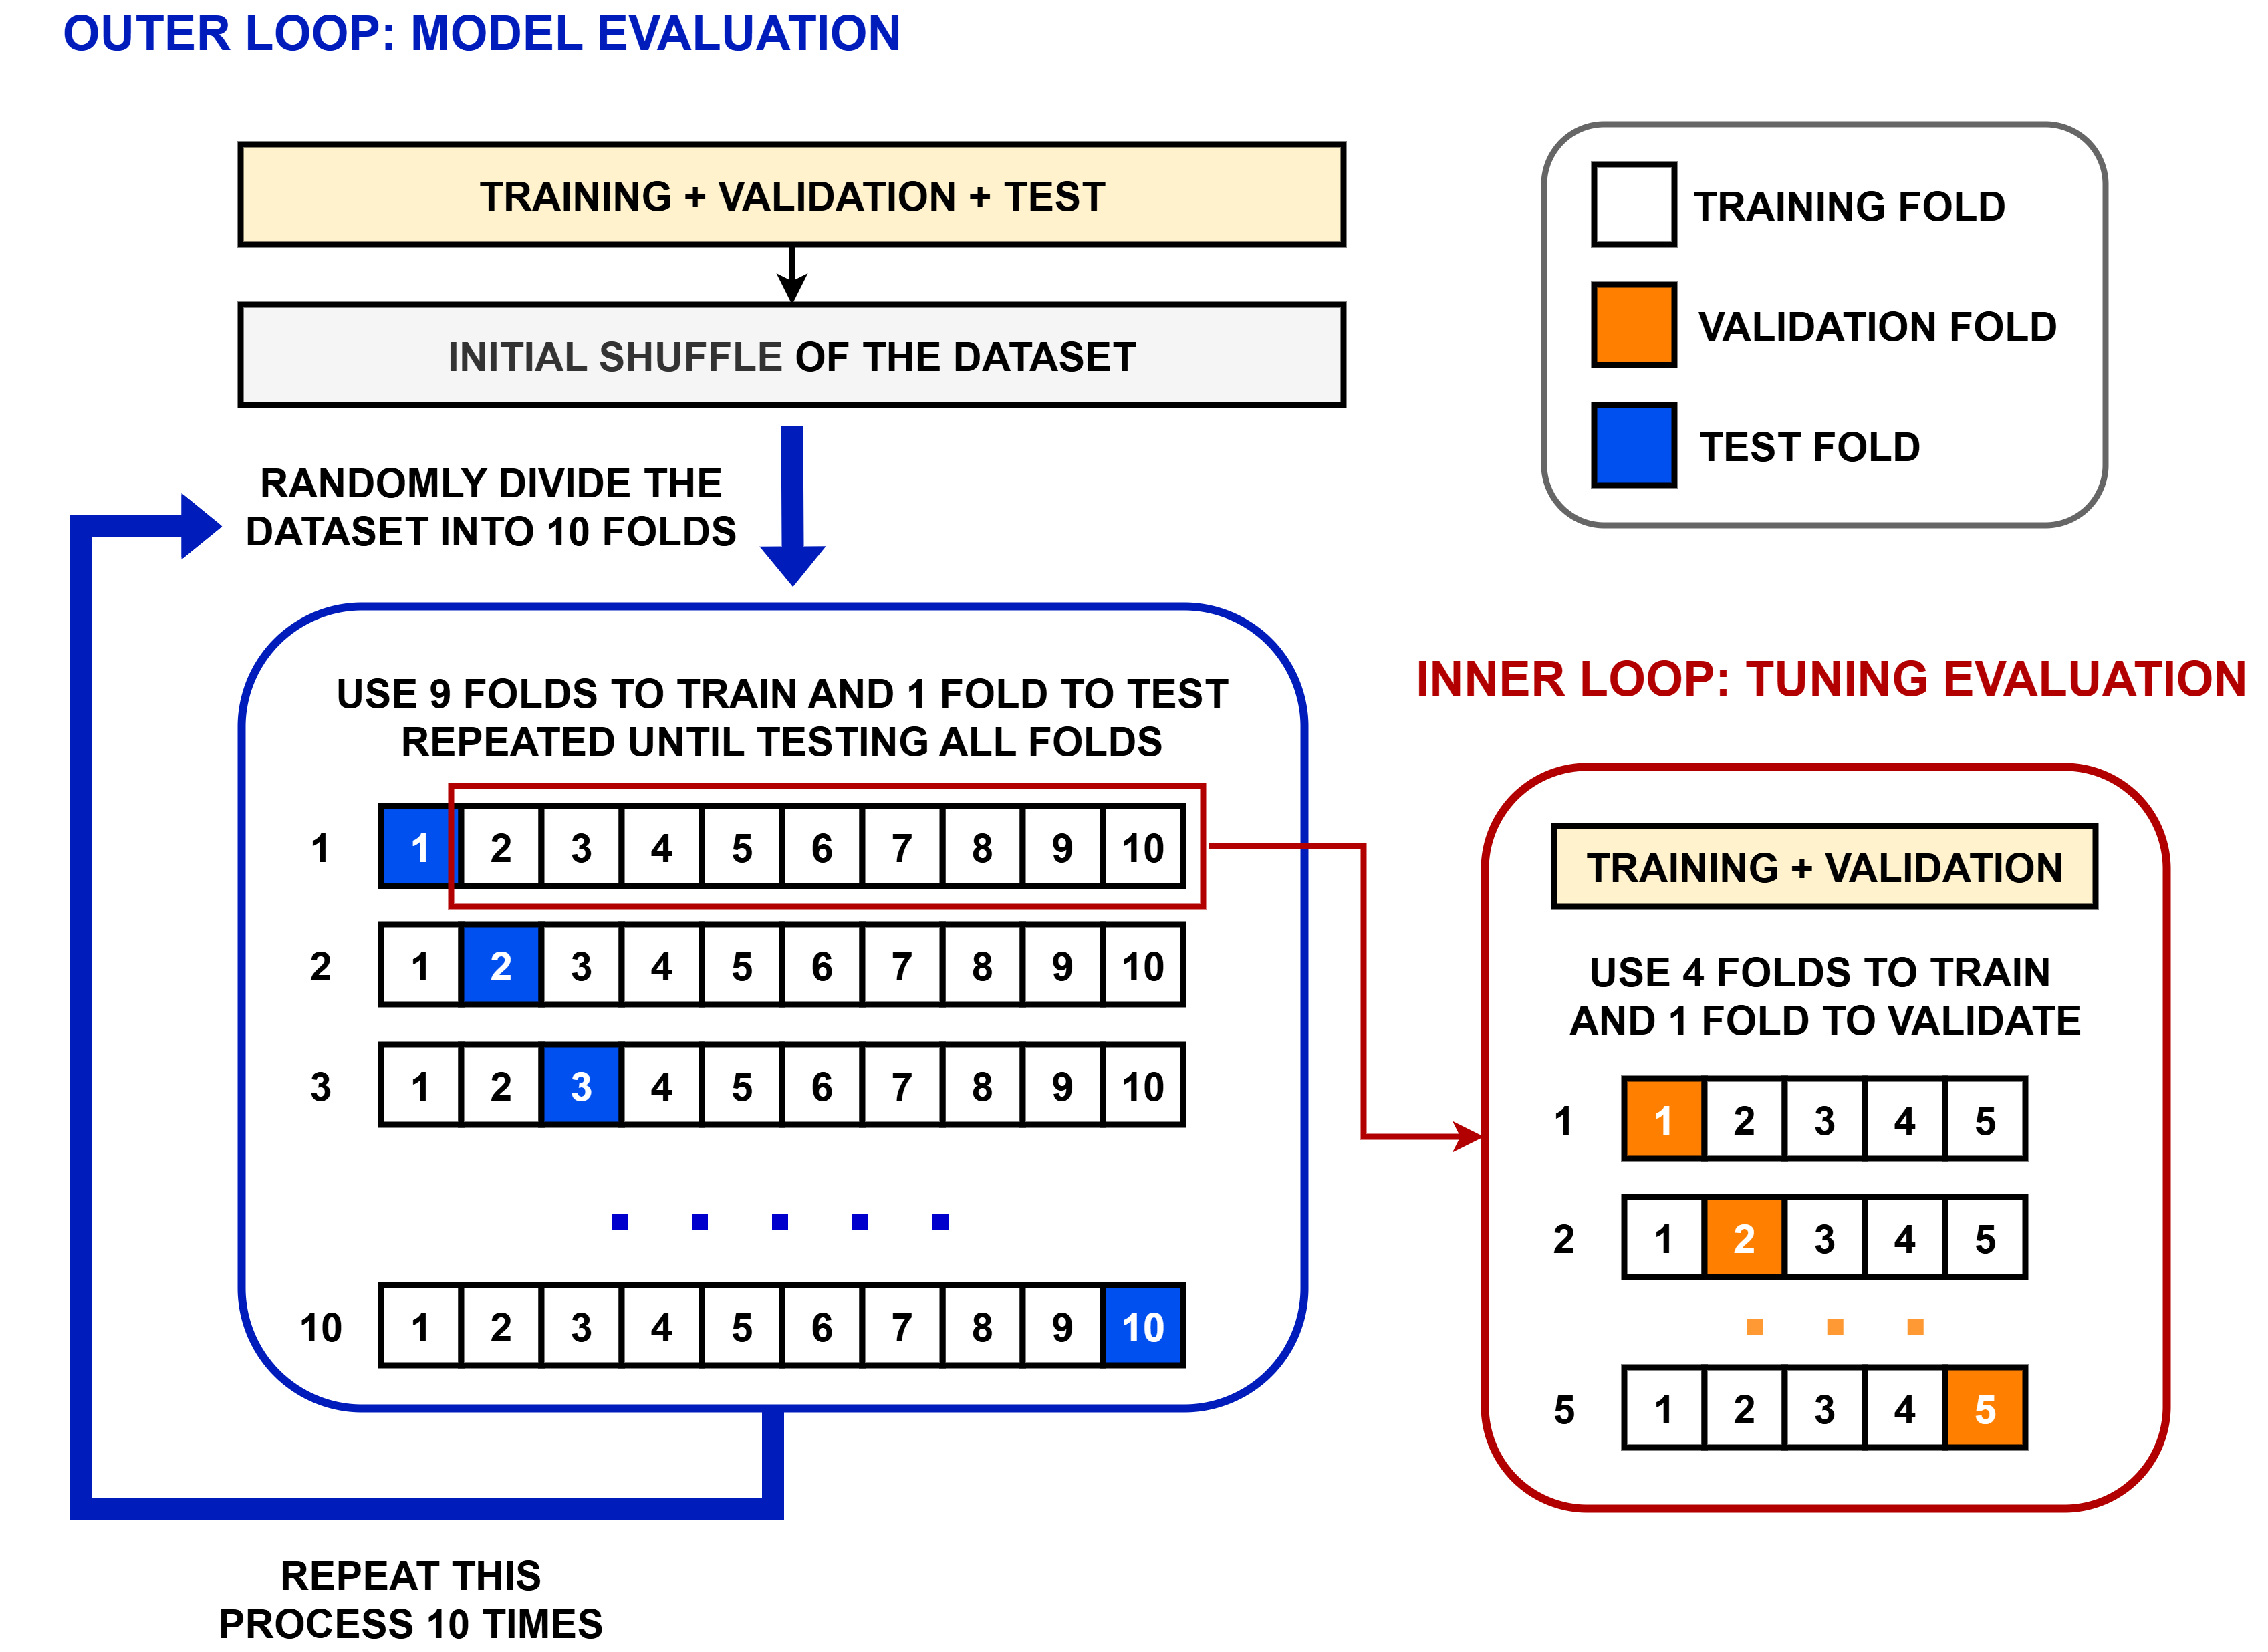
\includegraphics[width=\textwidth, height=0.65\textheight,keepaspectratio]{figures/10-times-10-fold-cv-schema-static.png}
        \end{column}
    \end{columns}

    % ================= BOTTOM SECTION: Full Width =================
    \begin{customexampleblock}{Model-Specific Data Split}
	Refitted on the full outer training set and evaluated on the test fold.
    \end{customexampleblock}

\end{frame}

%----------------------------------------------------------------------------------------

\begin{frame}
\frametitle{Learning Pipeline: Dynamic Ensembles}

    % ================= TOP SECTION: Two Columns =================
    \begin{columns} % [c] vertically centers the content in the columns
        
        % LEFT COLUMN: Concept and Math
        \begin{column}{0.35\textwidth}
    		\begin{customexampleblock}{Evaluation Protocol}
        		\begin{itemize}
            		\item \textbf{Evaluation (Outer Loop):} Repeated Stratified 10$\times$10 CV.
            		\item \textbf{Tuning (Inner Loop):} Stratified 5-Fold CV.
            		\item \textbf{Tuning Algorithm:} \texttt{Random Search} (\texttt{n\_iter=30}).
        		\end{itemize}
            \end{customexampleblock}
            
        \end{column}
        
        % RIGHT COLUMN: Visual Representation
        \begin{column}{0.60\textwidth}
		\centering
   		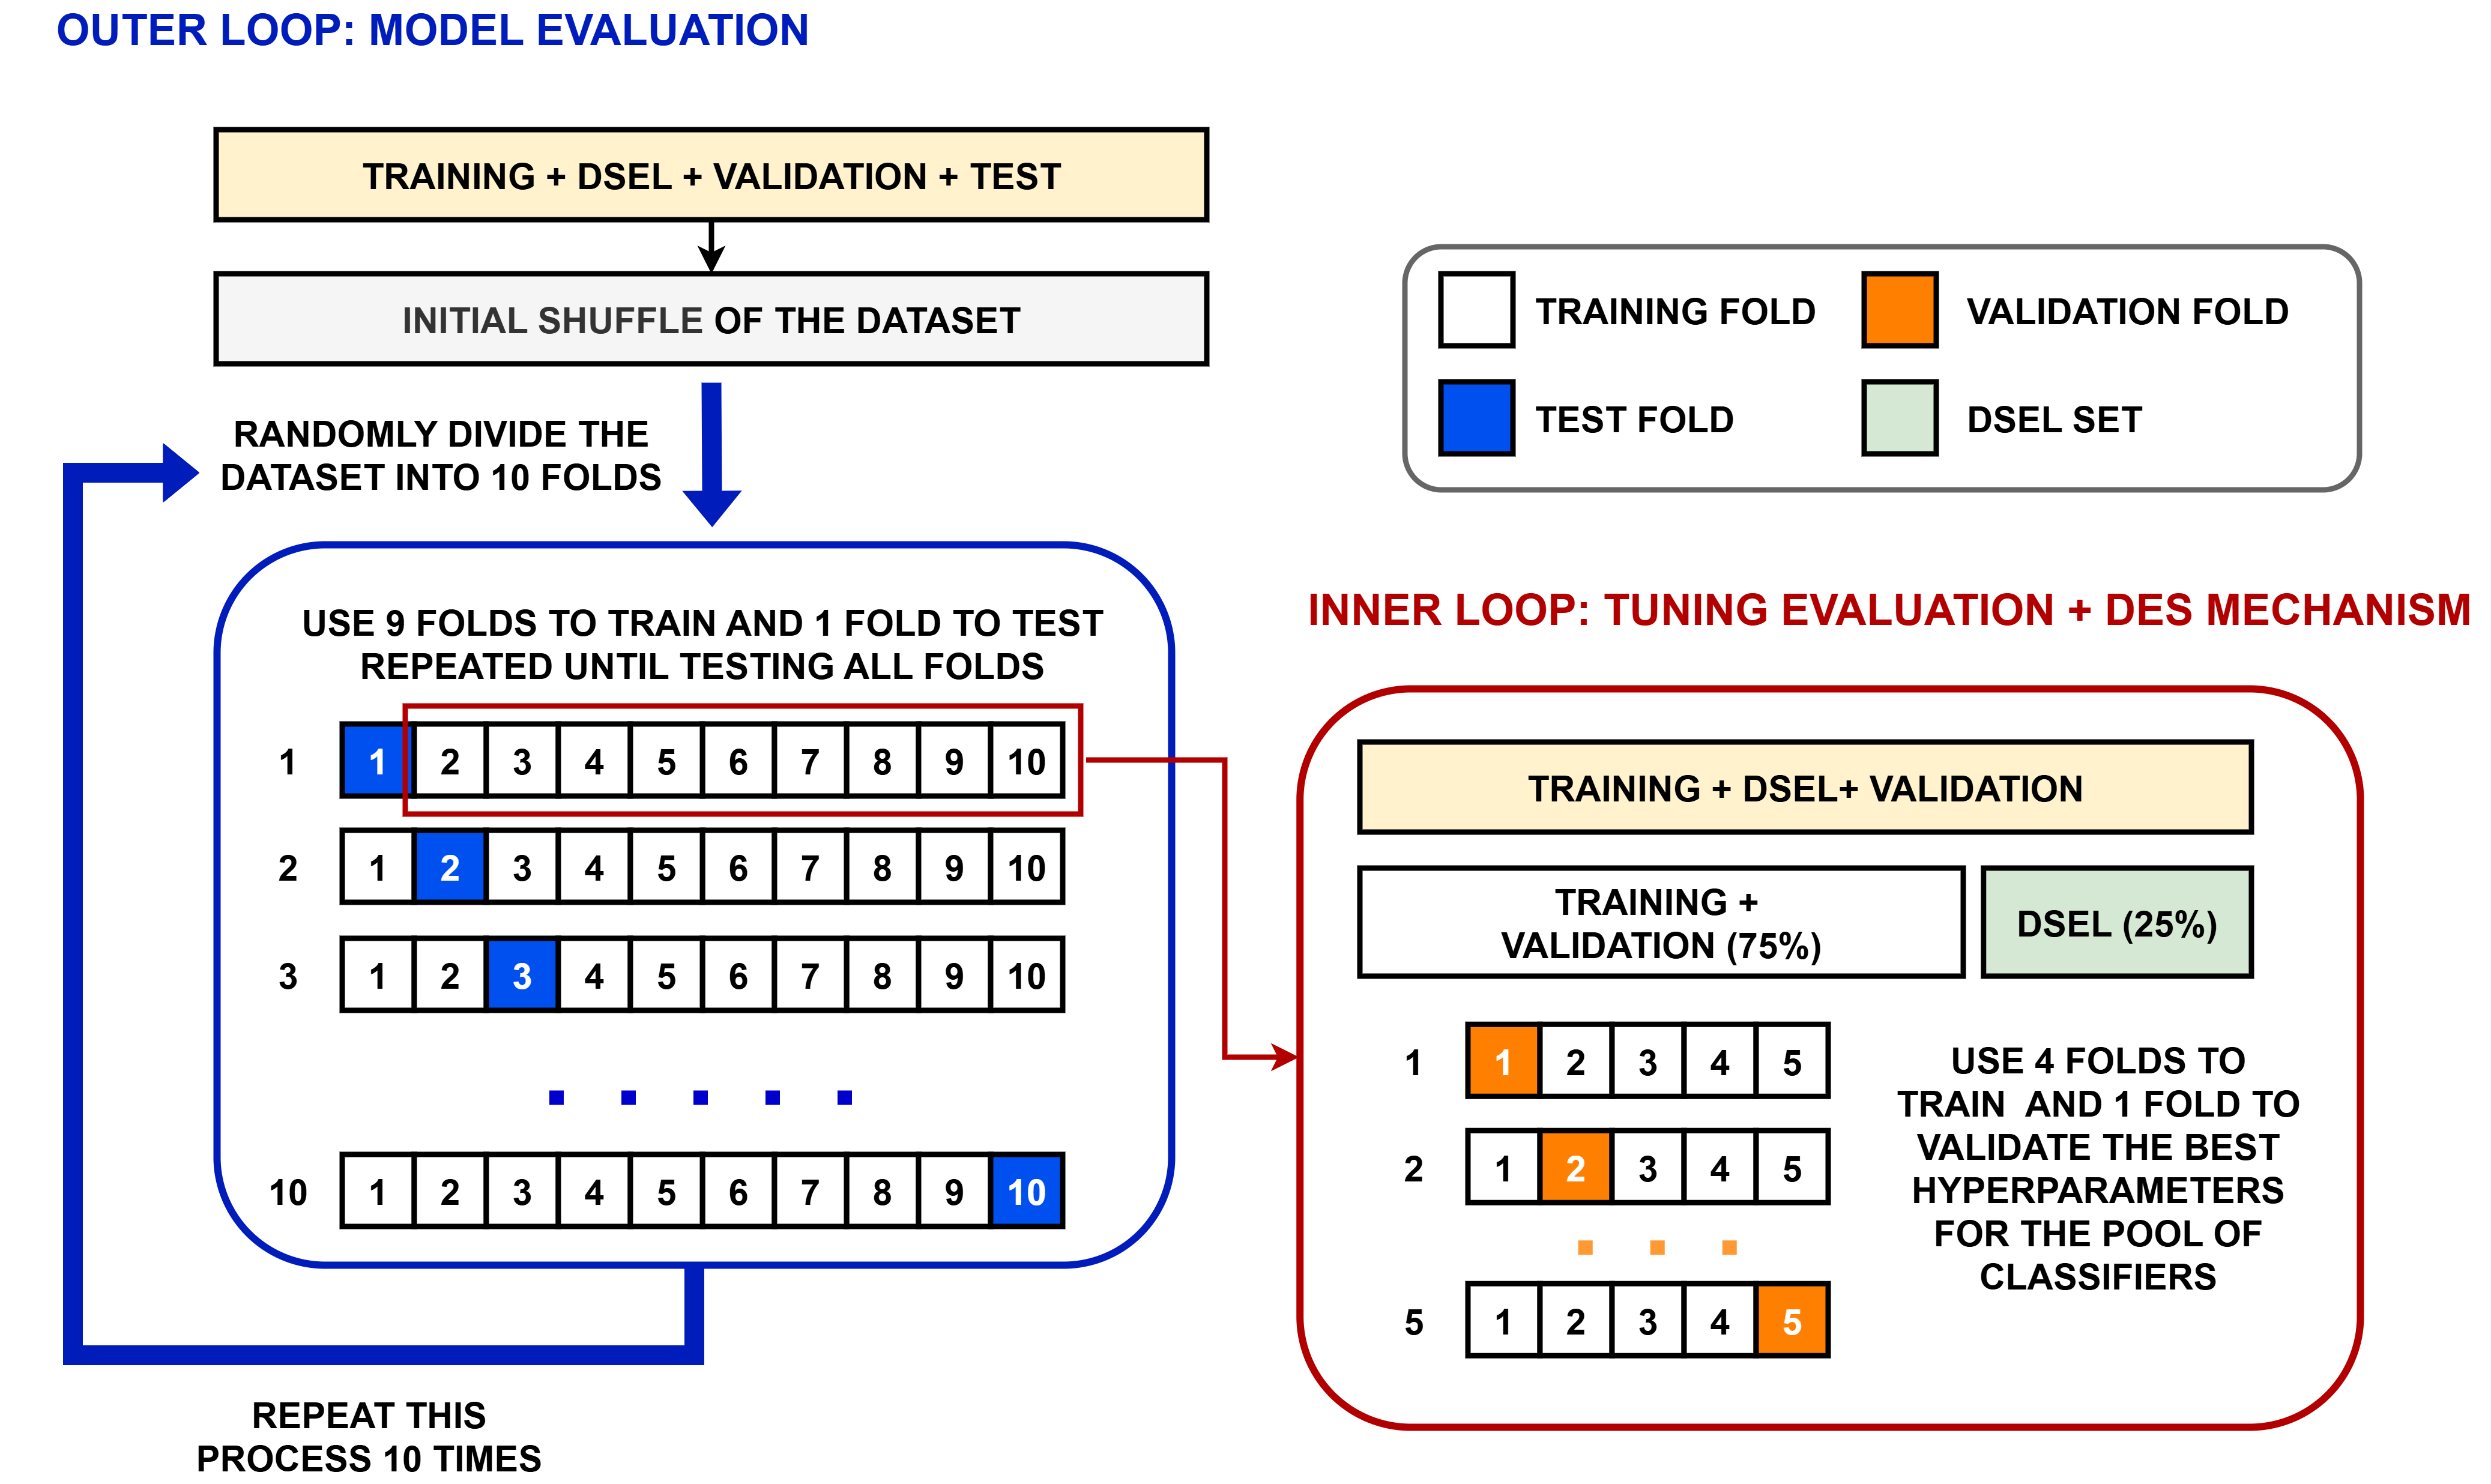
\includegraphics[width=\textwidth,keepaspectratio]{figures/10-times-10-fold-cv-schema-dynamic.png}
        \end{column}
        
    \end{columns}

    % ================= BOTTOM SECTION: Full Width =================
    \begin{customexampleblock}{Model-Specific Data Split}
	The outer training set requires a further split: \textbf{75\% (TRAIN)} to learn and tune the base classifier pool \textbf{25\% (DSEL)} to fit the competence estimation mechanism.
    \end{customexampleblock}

\end{frame}
%----------------------------------------------------------------------------------------

\begin{frame}
\frametitle{Evaluation Framework \& Metrics}
    \begin{customexampleblock}{Key Performance Metrics}
        \begin{itemize}
            \item \textbf{Standard Metrics:} Accuracy, Precision, Recall, F1-score, and ROC-AUC to get a general overview of discriminative power.
            \item \textbf{Primary Metric - Average Cost (\texttt{AvgCost}):} A domain-specific Average Cost per Prediction that directly quantifies asymmetric clinical risk.
        \end{itemize}
    \end{customexampleblock}
    
    \begin{center}
        \Large \texttt{AvgCost} = $\frac{\textbf{1} \;\cdot\; \text{FP} \;+\; \textbf{10} \;\cdot\; \text{FN}}{N}$
        \\ \vspace{0.5em}
        \small (\textit{Lower is better})
    \end{center}
    
    \begin{customexampleblock}{Statistical Validation}
		\begin{itemize}
            \item We applied the \textbf{corrected resampled t-test} on the \texttt{AvgCost} metric to rigorously compare model configurations.
            \item A p-value < $0.05$ was used to determine statistically significant differences.
        \end{itemize}
    \end{customexampleblock}

\end{frame}

%========================================================================================
\section{Results and Discussion}
%========================================================================================
\begin{frame}
\frametitle{Results: Baseline \& Imbalance Bottleneck}

    \begin{center}
        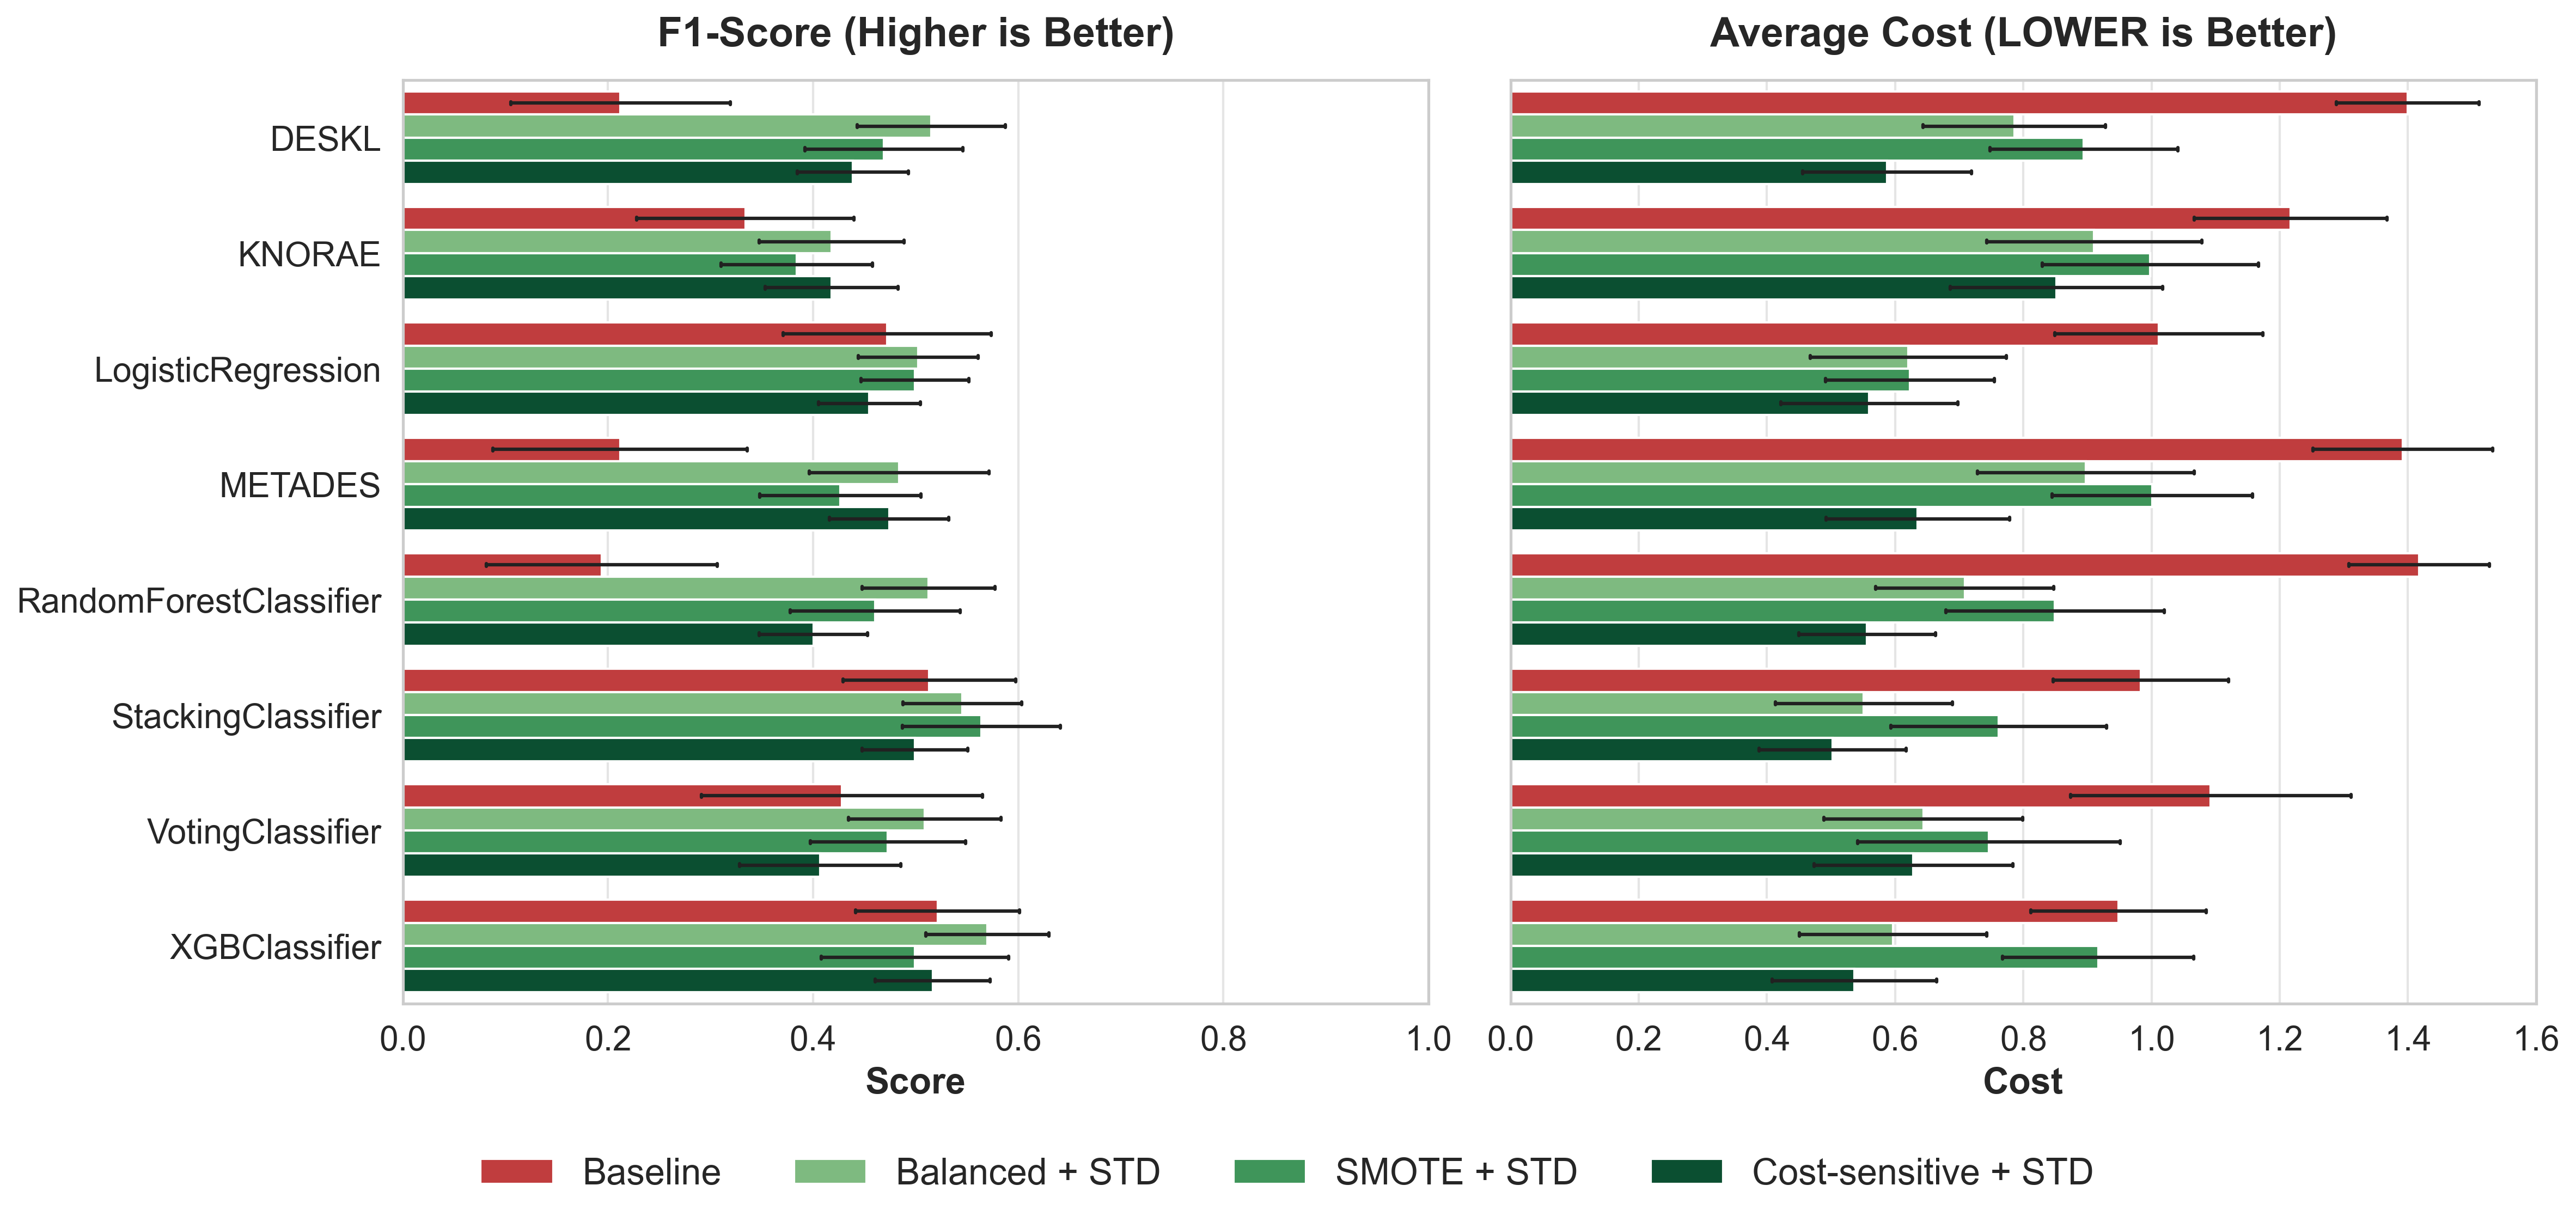
\includegraphics[width=\textwidth, height=0.7\textheight,keepaspectratio]{figures/slide1_baseline_std_settings_f1_average_cost.png}
    \end{center}
    
    \begin{itemize}
    	\item \textbf{Baseline} setting yields unacceptable \textbf{AvgCost} due to extreme class imbalance.
        \item Introducing \textbf{Imbalance-Aware} methods drastically reduces the  \textbf{AvgCost}.
		\end{itemize}
  
\end{frame}

%----------------------------------------------------------------------------------------

\begin{frame}
\frametitle{Results: The MEC Performance}

    \begin{center}
        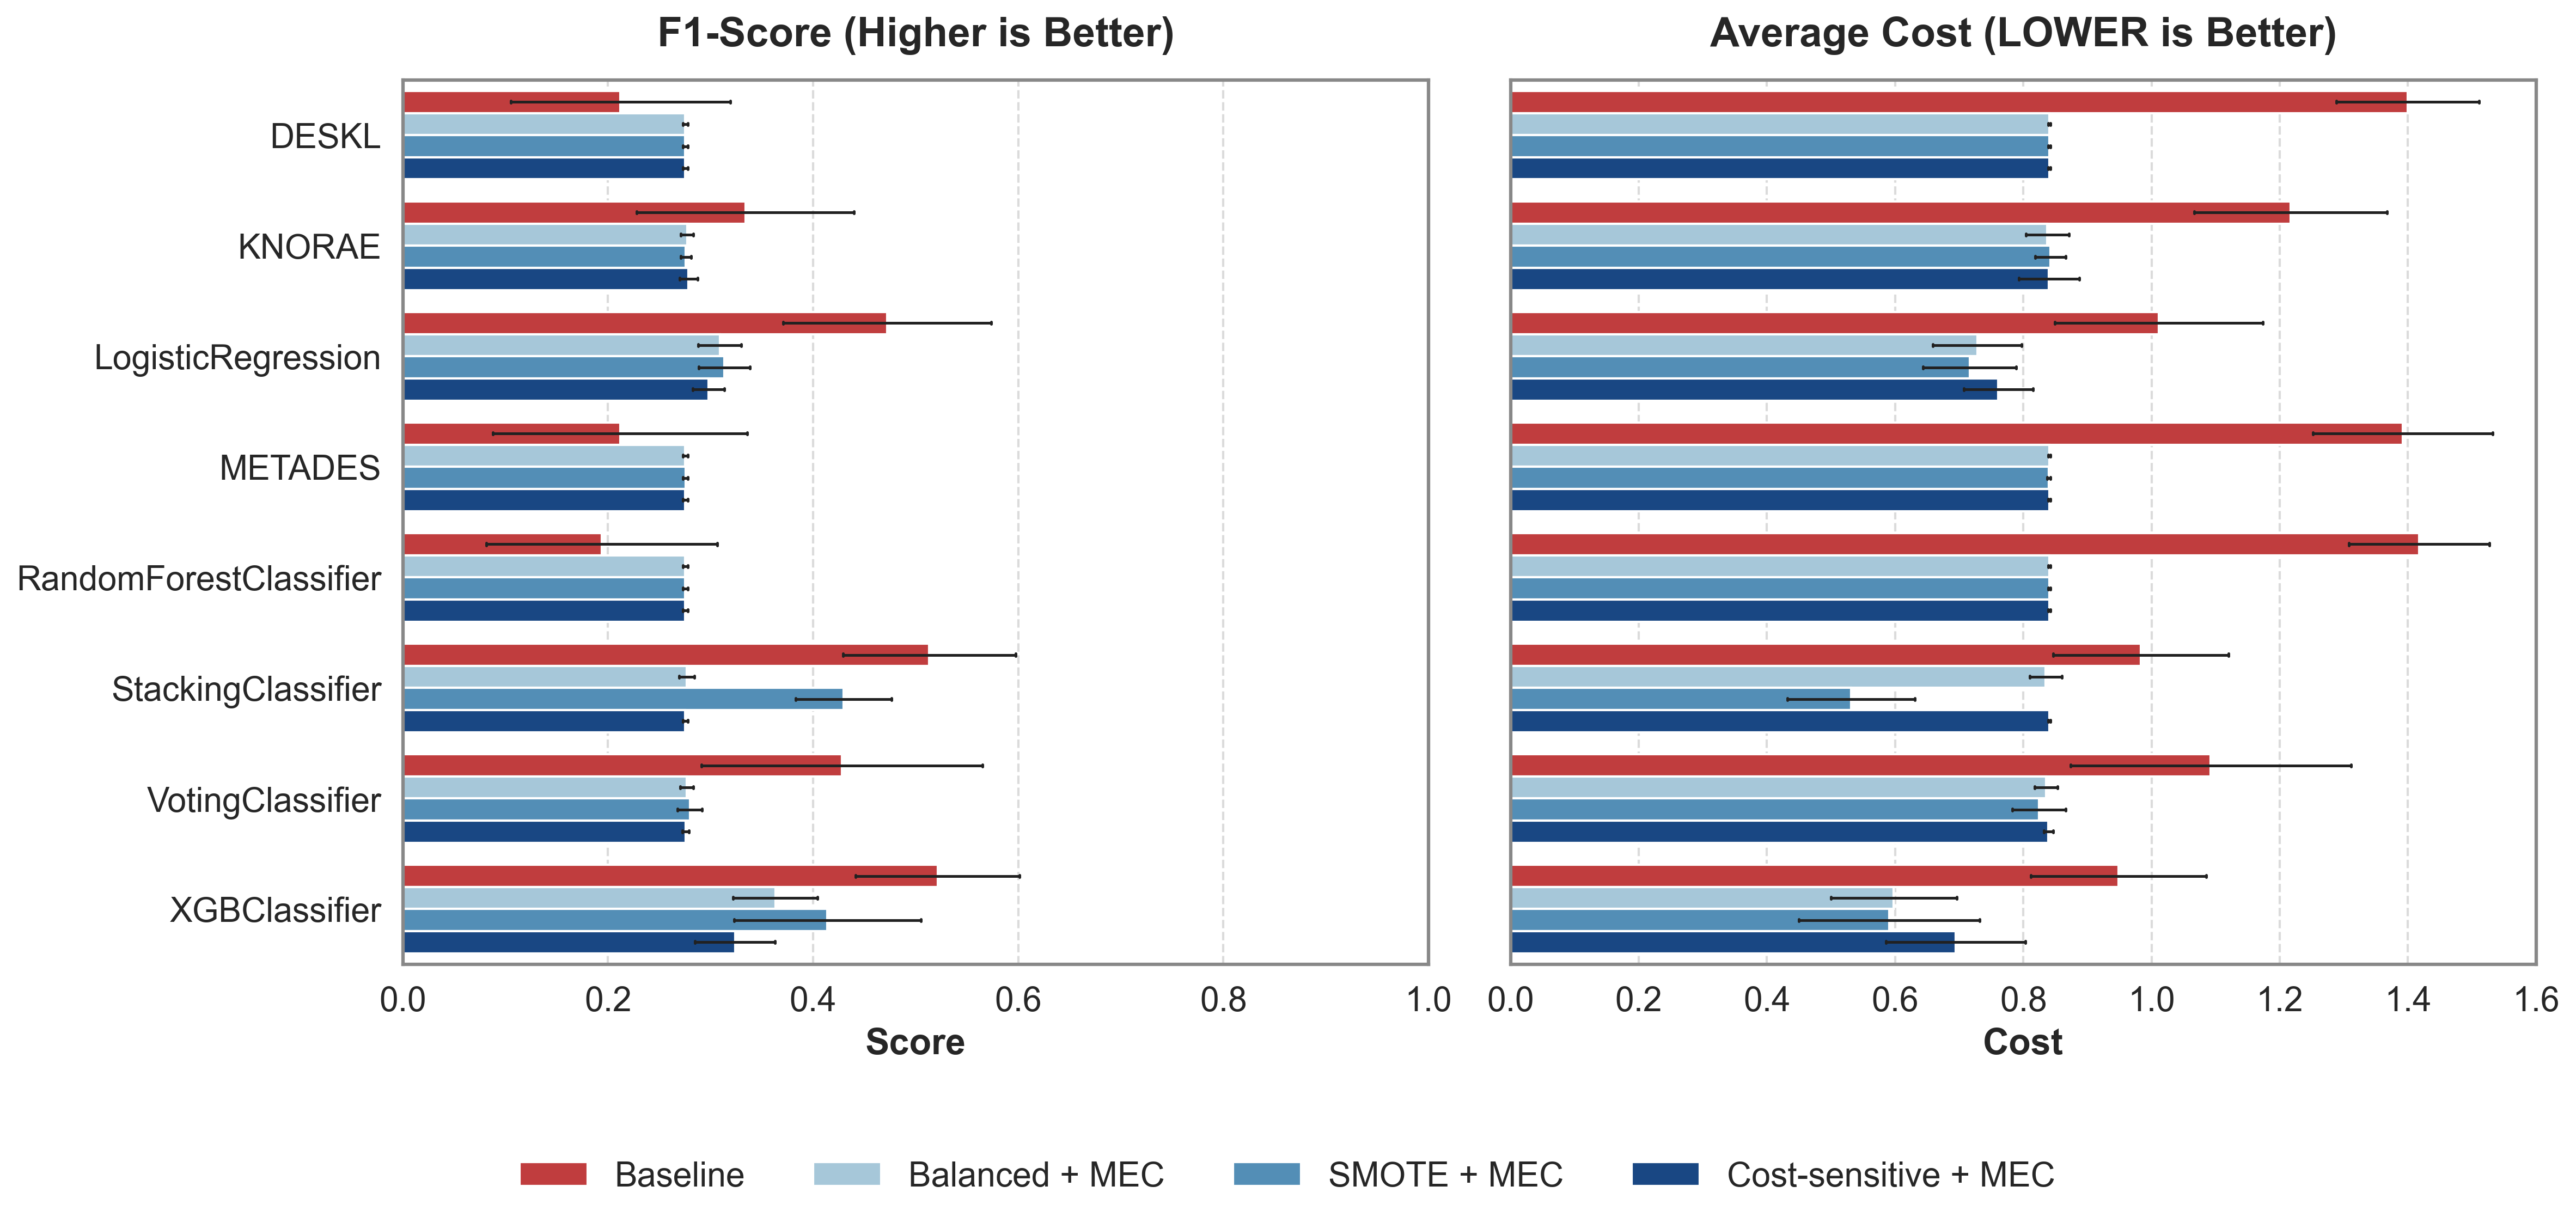
\includegraphics[width=\textwidth, height=0.7\textheight,keepaspectratio]{figures/slide2_baseline_mec_settings_f1_average_cost.png}
    \end{center}
    
    \begin{itemize}
    	\item Applying the \textbf{MEC} threshold successfully drives the \textbf{AvgCost} down.
		\item The overall \textbf{F1-Score stalls} or even degrades across all architectures.
	\end{itemize}

\end{frame}

%----------------------------------------------------------------------------------------

\begin{frame}
\frametitle{Results: The Precision-Recall Trade-off}

    \begin{center}
        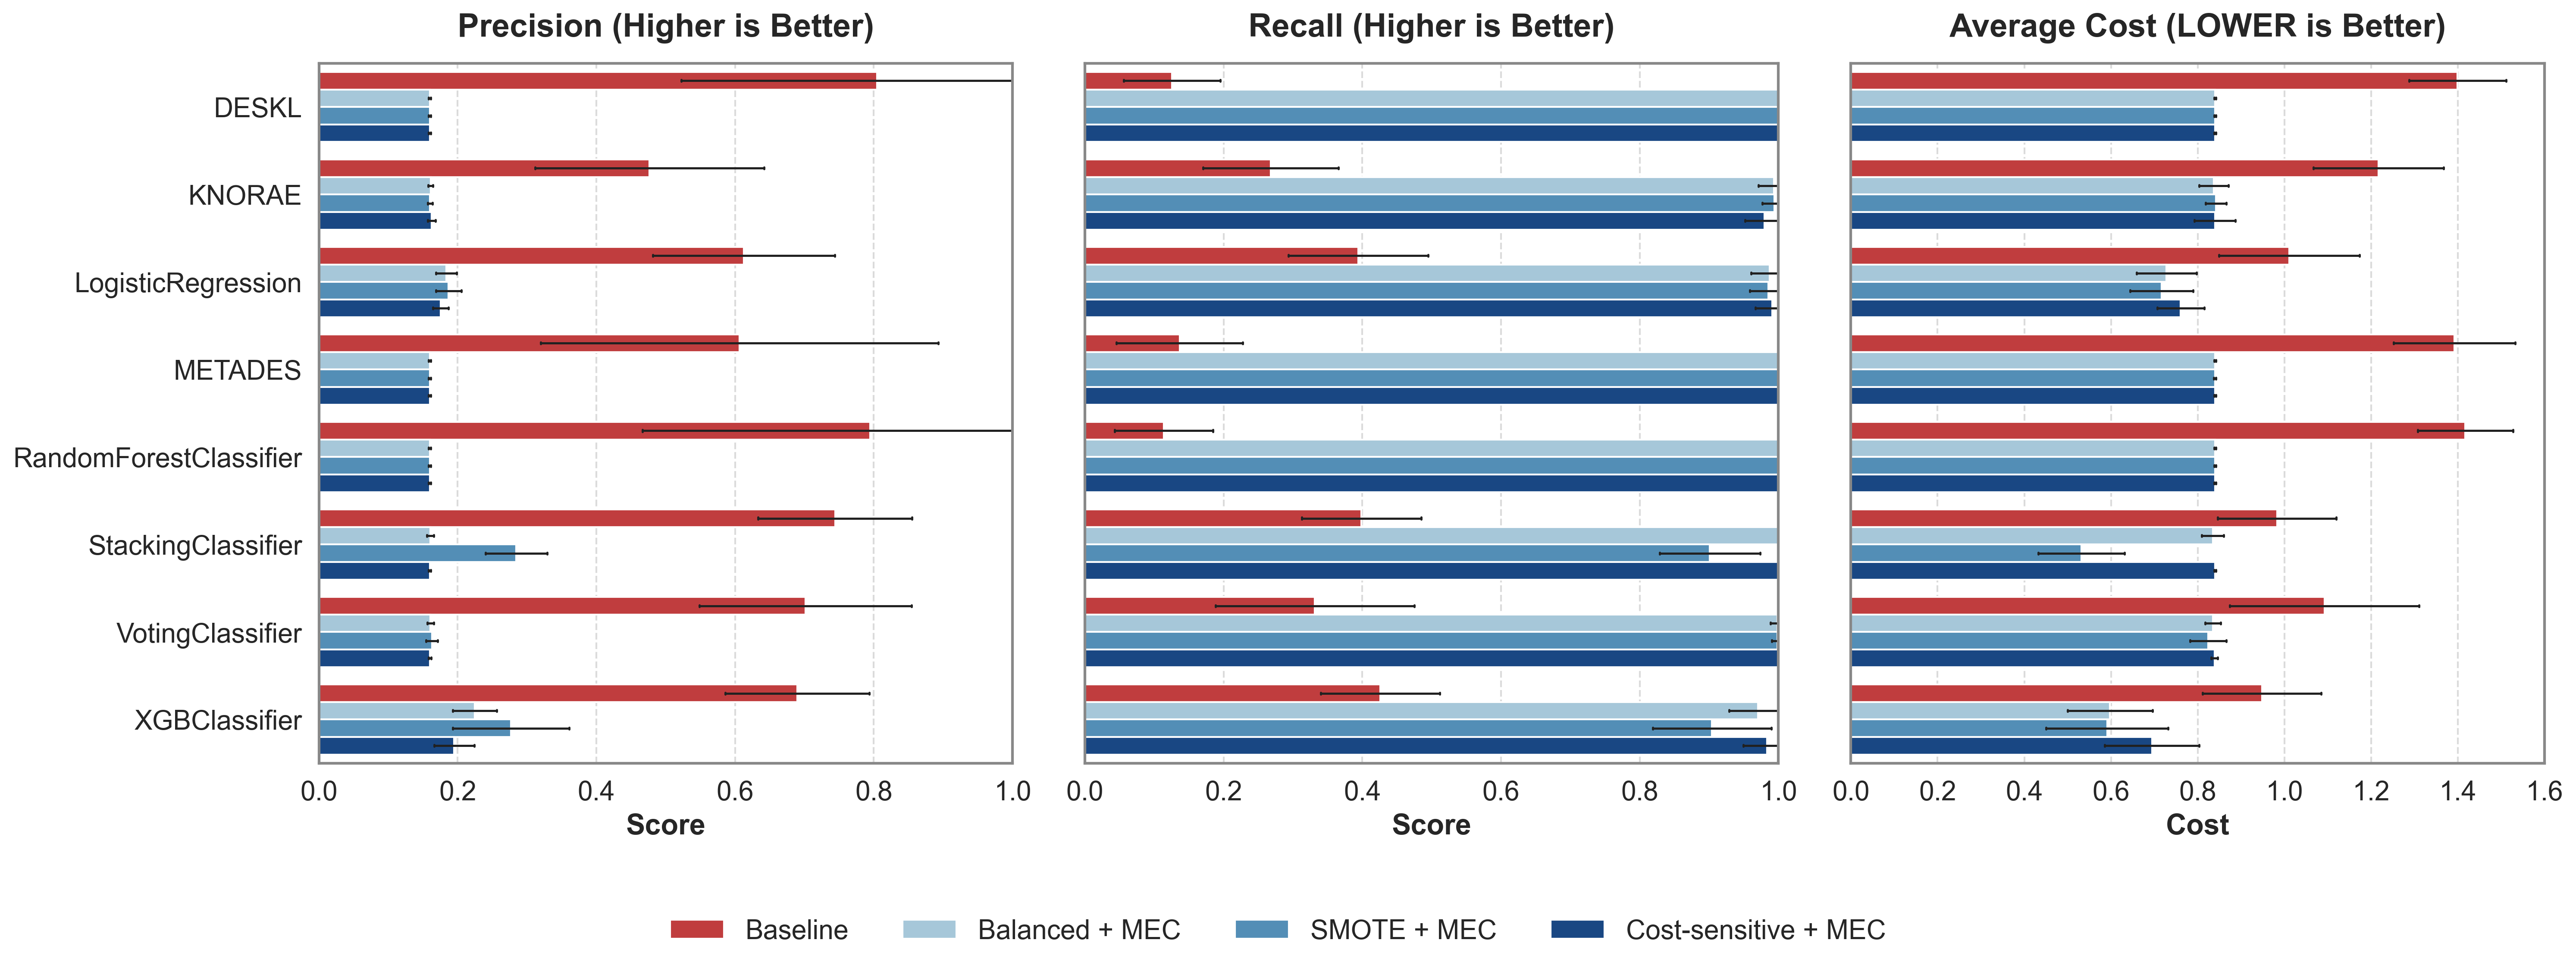
\includegraphics[width=\textwidth,keepaspectratio]{figures/slide2_baseline_mec_settings_precision_recall_average_cost.png}
    \end{center}
    
    \begin{itemize}
    	\item To minimize the expected cost, the model pushes \textbf{Recall} near 1.0, eliminating FN.
    	\item Consequently, this extreme sensitivity causes \textbf{Precision} to drop. The model over-predicts the minority class, generating numerous FP that penalize the F1-Score.
	\end{itemize}

\end{frame}

%----------------------------------------------------------------------------------------

\begin{frame}
\frametitle{Results: Imbalance-Aware Settings + Standard Threshold}

    \begin{center}
        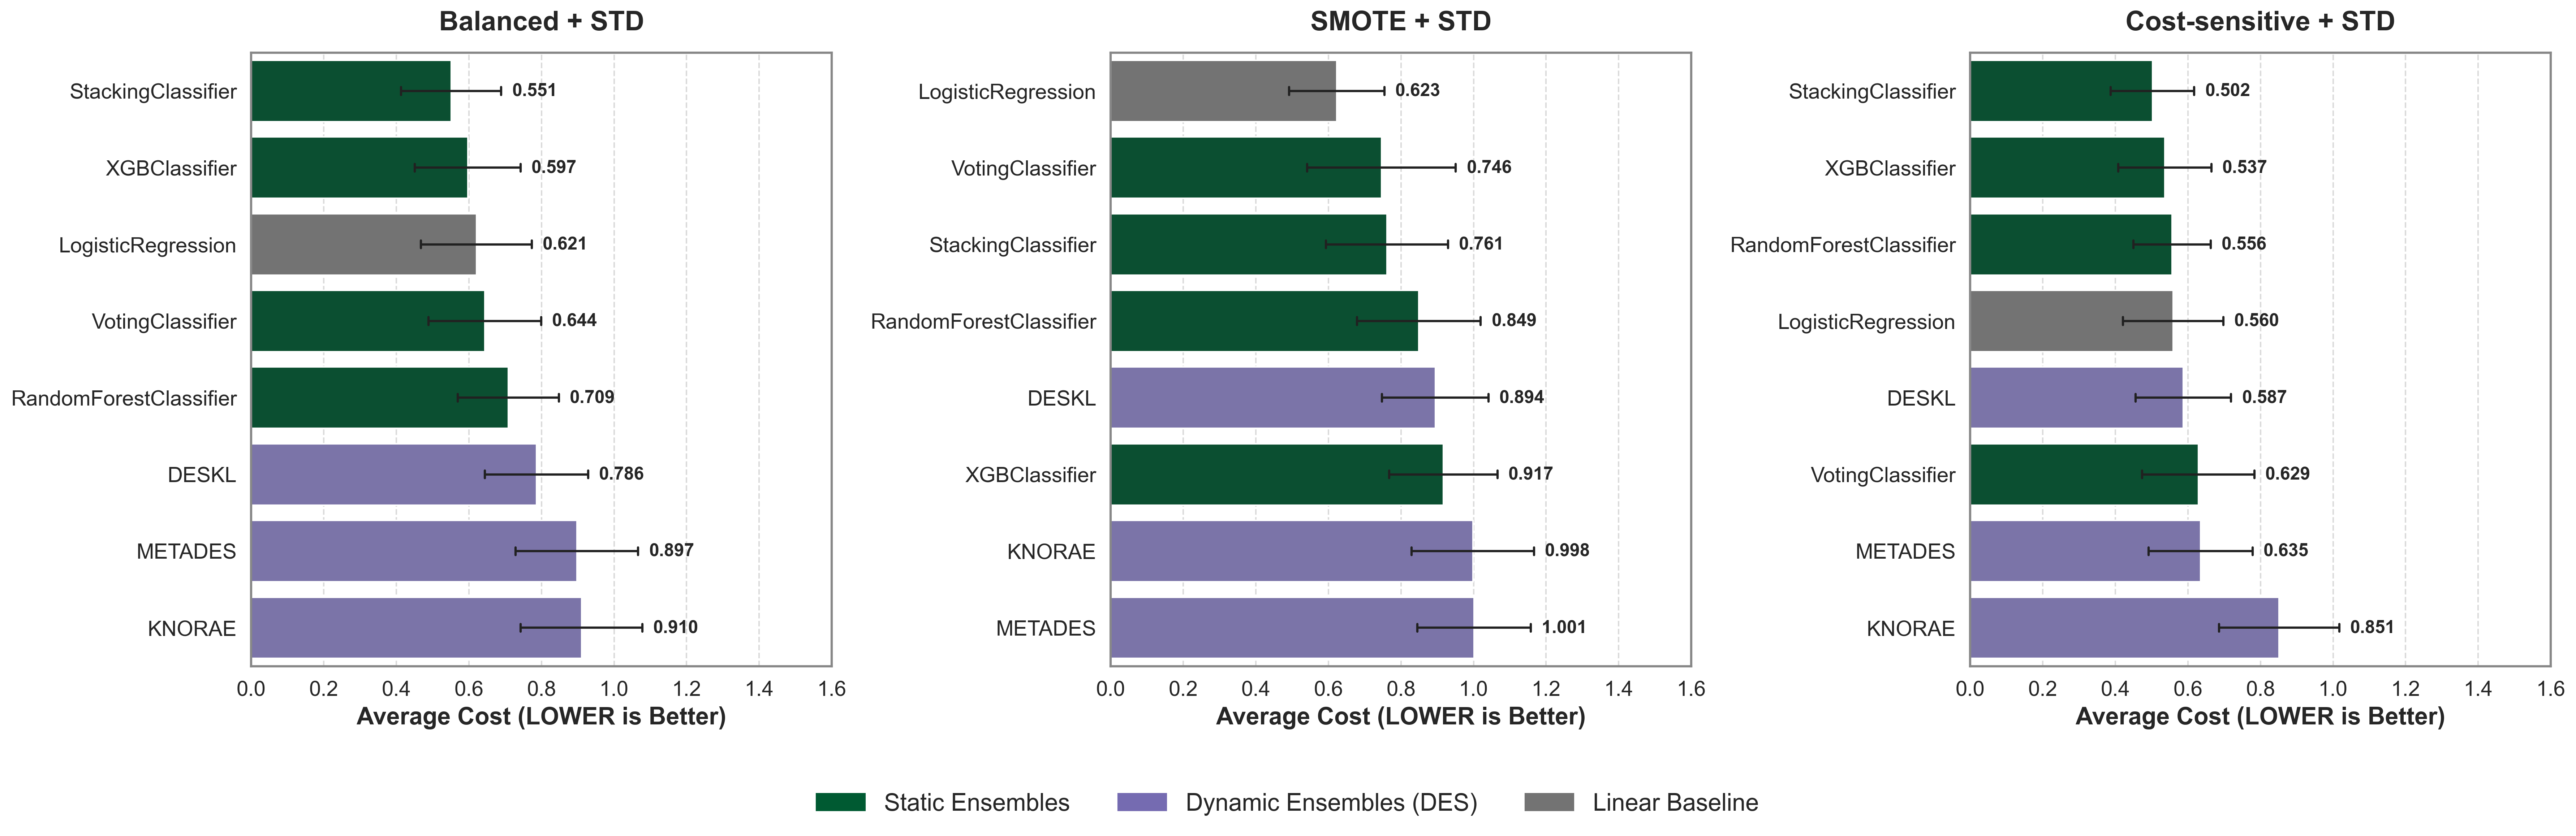
\includegraphics[width=\textwidth,keepaspectratio]{figures/slide4_std_settings_static_des_average_cost.png}
    \end{center}
    
    \begin{itemize}
    	\item Linear models struggle with the dataset's non-linearity and imbalance.
    	\item Static and Dynamic Ensembles consistently reduce the AvgCost, proving their necessity for modeling complex clinical data.
    \end{itemize}

\end{frame}

%----------------------------------------------------------------------------------------

\begin{frame}
\frametitle{Results: Imbalance-Aware Settings + MEC}

    \begin{center}
        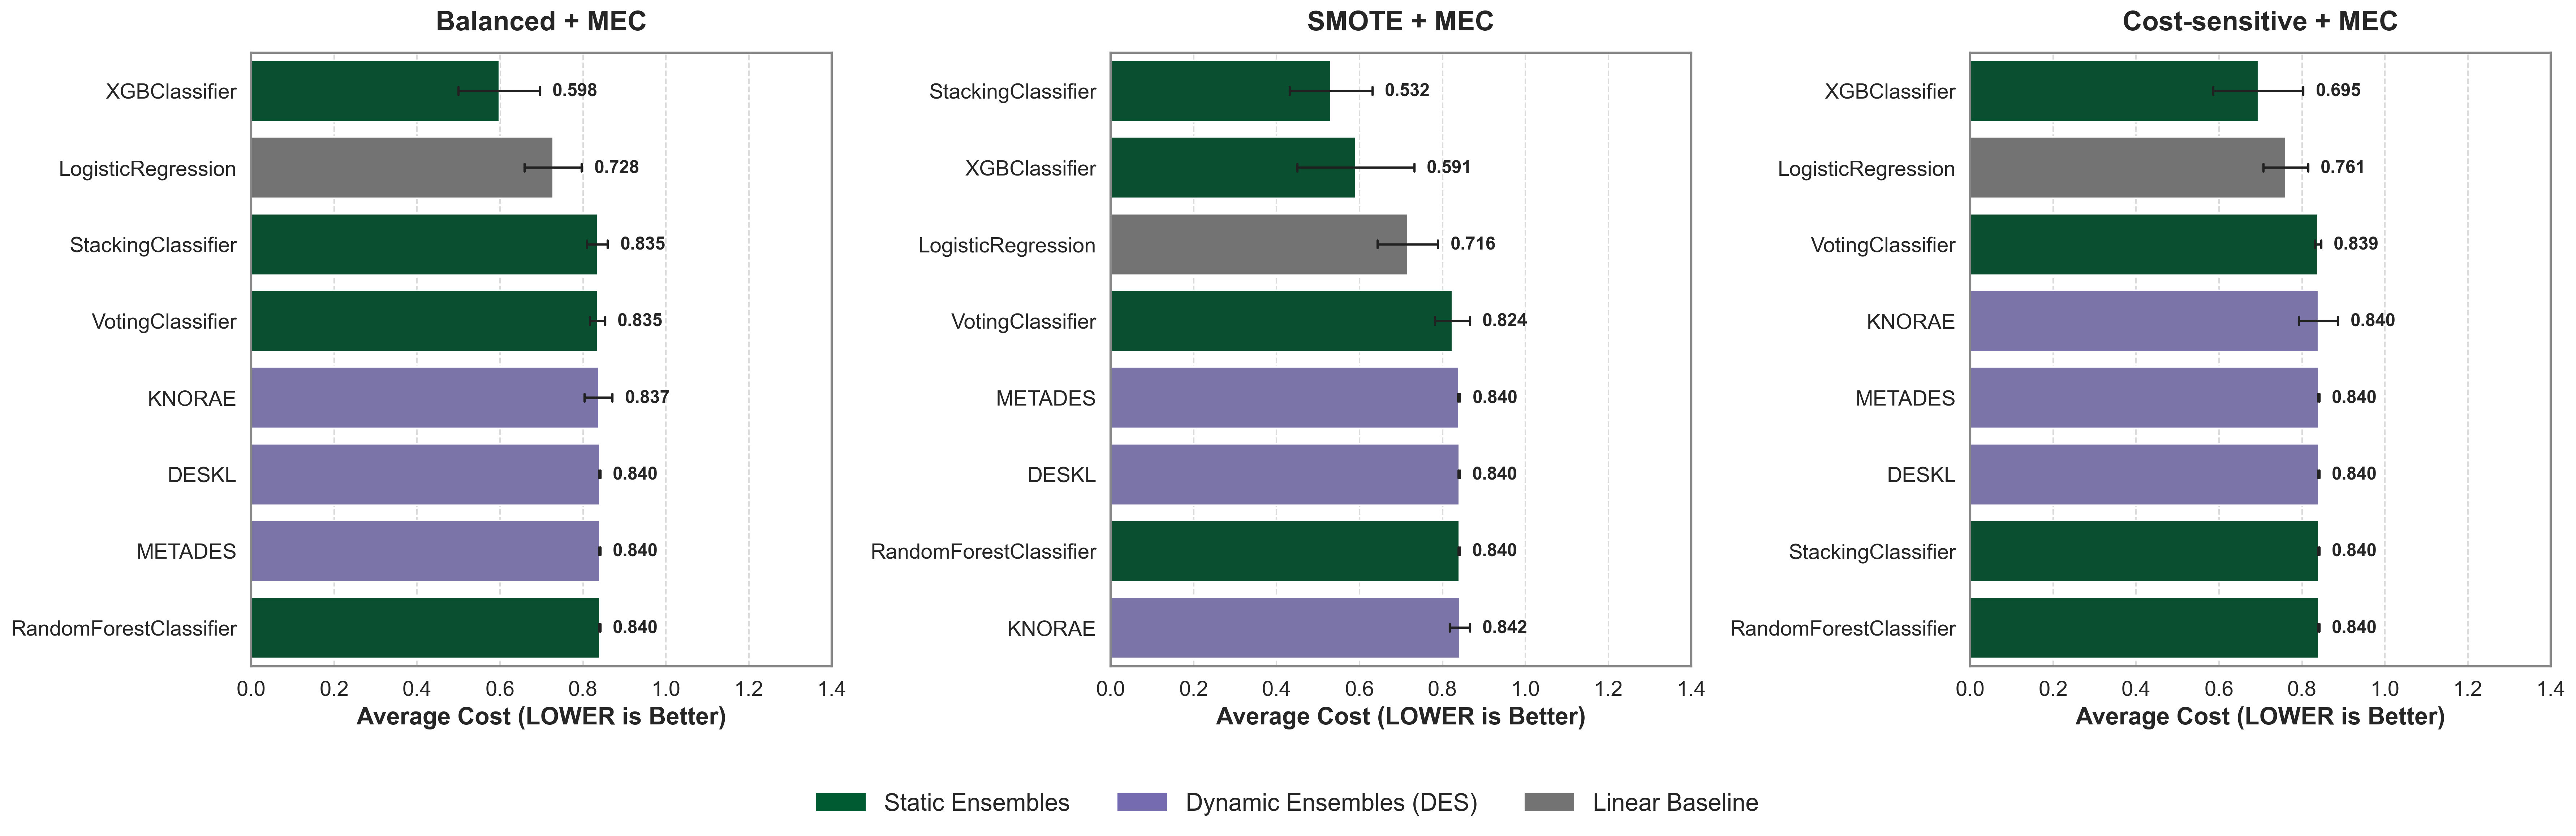
\includegraphics[width=\textwidth,keepaspectratio]{figures/slide4_mec_settings_static_des_average_cost.png}
    \end{center}
    
    \begin{itemize}
    	\item The aggressive MEC threshold compresses the performance gap across all families.
    	\item \textbf{Stacking} (Static) maintains the absolute minimum AvgCost, slightly outperforming the local $k$-NN competence regions relied upon by DES.
    \end{itemize}

\end{frame}

%----------------------------------------------------------------------------------------

\begin{frame}
\frametitle{Results: Global Benchmarking (The Top 10 Models)}

    % ================= TOP SECTION: Two Columns =================
    \begin{columns}
        \begin{column}{0.68\textwidth}
        	\centering
   			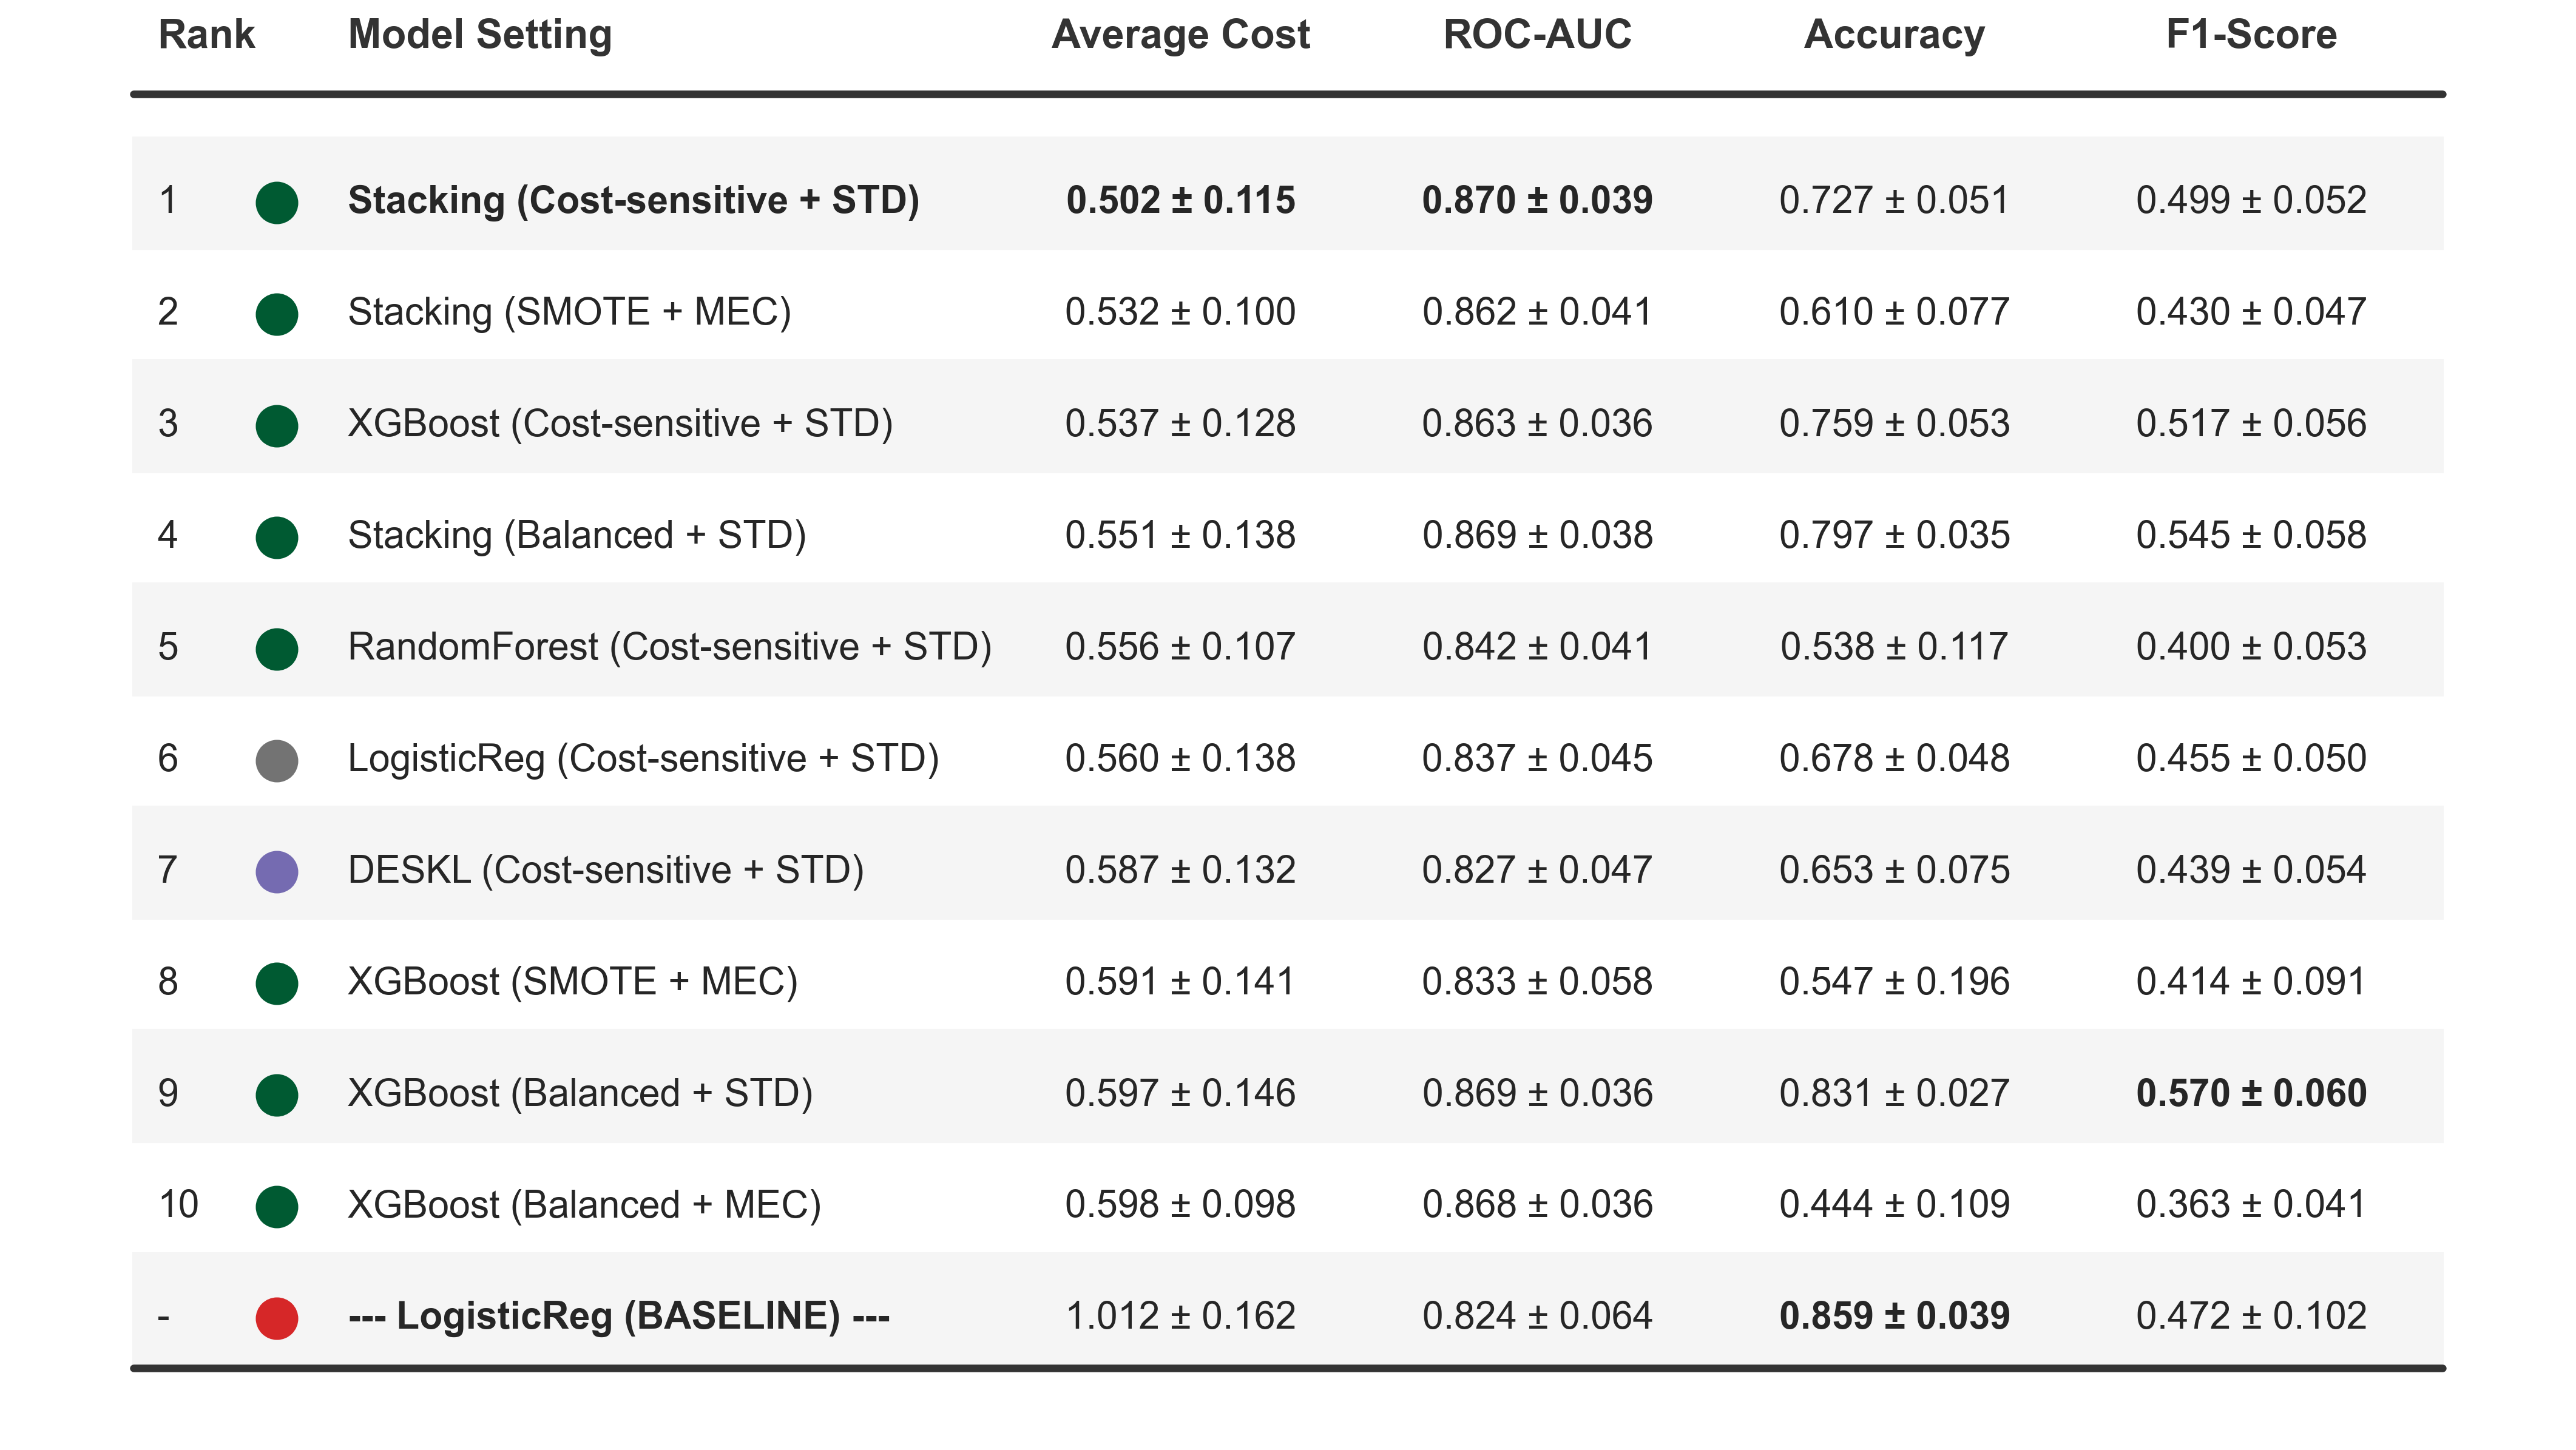
\includegraphics[width=\textwidth,keepaspectratio]{figures/slide5_final_table_metrics.png}
        \end{column}
        
        \begin{column}{0.40\textwidth}
        -- The \textbf{Top 10} features 5 different architectures (Stacking, XGBoost, RF, LogReg, DES). \\
        \vspace{0.5em}
        -- \textbf{Stacking (Rank 1)} reaches the minimum AvgCost (0.502). \\
        \vspace{0.5em}
        -- \textbf{XGBoost (Rank 9)} reaches an higher AvgCost (0.597) with a superior F1-Score (0.570).

        \end{column}        
    \end{columns}

    % ================= BOTTOM SECTION: Full Width =================
    \vspace{0.5em}
	Rank 1 wins on strict cost, but Rank 9 offers a much better diagnostic balance: \\ \textbf{is the cost difference between 0.502 and 0.597 actually statistically significant?}

\end{frame}

%----------------------------------------------------------------------------------------

\begin{frame}
\frametitle{Results: Global Benchmarking (The Top 10 Models)}

    % ================= TOP SECTION: Two Columns =================
    \begin{columns}
        \begin{column}{0.60\textwidth}
        	\centering
   			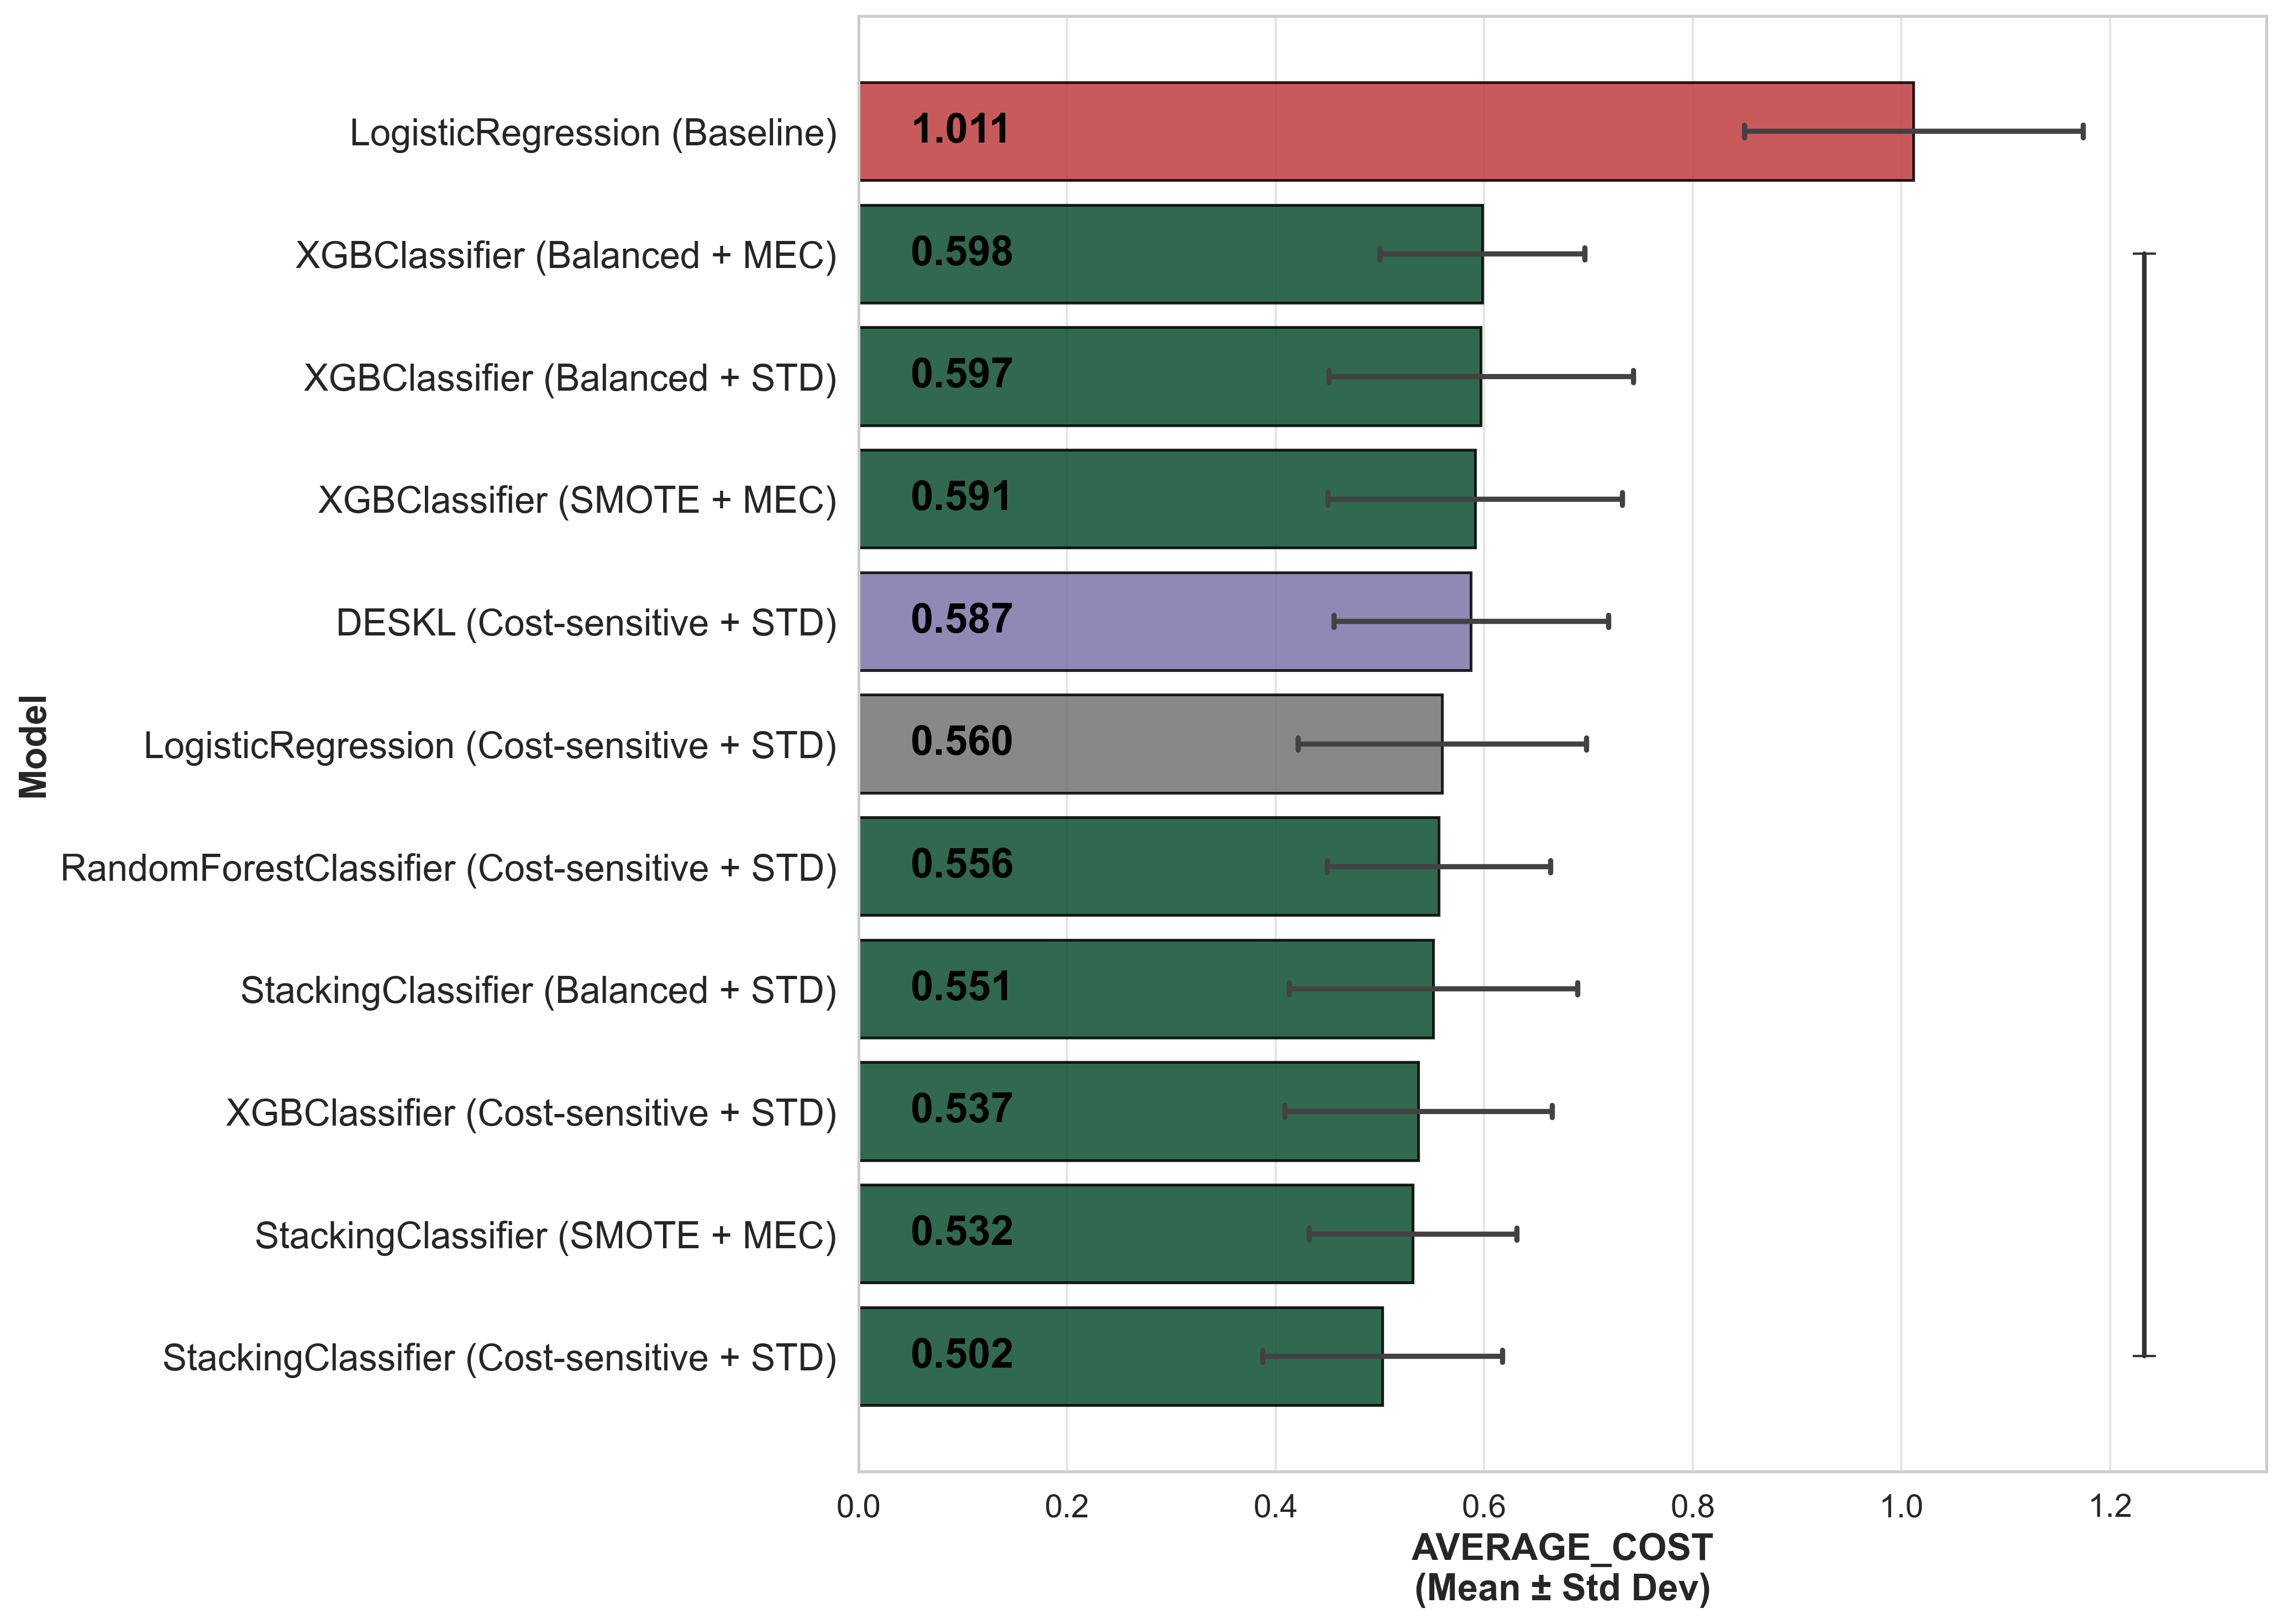
\includegraphics[width=\textwidth,height=0.80\textheight,keepaspectratio]{figures/slide5_top10_corrected_resampled_ttest_average_cost_barplot_significance.png}
        \end{column}
        
        \begin{column}{0.40\textwidth}
        -- T-test confirms that Top 10 models are statistically superior to the linear baseline in AvgCost. \\
        
        \vspace{0.5em}
        -- However, these 10 models are not statistically different from one another in AvgCost. \\
        
        \vspace{0.5em}
        -- We must pivot to secondary metrics (\textbf{ROC-AUC} and \textbf{F1-Score}) to make a final decision.

        \end{column}        
    \end{columns}

    % ================= BOTTOM SECTION: Full Width =================
    \vspace{0.3em}
	\textbf{XGBoost (Balanced + STD)} at Rank 9 keeps the same statistical cost as the Rank 1 model, reaching an \textbf{F1-Score of 0.570} and a highly robust \textbf{ROC-AUC of 0.869}.

\end{frame}

%========================================================================================
\section{Conclusions \& Future Directions}
%========================================================================================

\begin{frame}
\frametitle{Conclusions \& Future Directions}

	\textbf{Key Findings}
\begin{itemize}
            \setlength{\itemsep}{0.5em}
            \item Explicitly addressing class imbalance is crucial. \textbf{Cost-sensitive learning combined with a standard decision threshold} emerged statistically as the most reliable overall strategy, significantly beating raw baselines.
            
            \item The Minimum Expected Cost (MEC) rule does not provide a uniform advantage. Instead, it drives different models toward a converging operating behavior characterized by extremely high recall and collapsing precision.
            
            \item Static ensemble models, particularly \texttt{StackingClassifier} and \texttt{XGBClassifier}, proved to be the most robust architectures. They systematically outperformed the most competitive dynamic method (\texttt{DESKL}) in this specific context.
            
            \item The statistical equivalence among the top static ensembles allows clinicians to safely select models like \texttt{XGBoost} that balance the lowest clinical penalty with superior diagnostic precision (F1-Score).
        \end{itemize}
\end{frame}

%----------------------------------------------------------------------------------------

\begin{frame}
\frametitle{Conclusions \& Future Directions}

	\textbf{Limitations \& Future Works}
	\begin{itemize}
	    \setlength{\itemsep}{0.5em}

		\item The current dataset originates from an older, relatively limited clinical context. Future work must extend this analysis to contemporary, large-scale dataset to guarantee modern clinical applicability.
            
            \item The current framework predicts binary mortality strictly at admission time. Subsequent research should expand this pipeline to predict specific causes of death, non-lethal complications, and dynamic risks at later hospitalization stages.
            
            \item The evaluated DES methods do not exhaust the dynamic selection literature. Future studies should investigate alternative pool-generation strategies and conduct \textbf{dedicated threshold calibration} (beyond MEC) to optimally manage the FP vs. FN trade-off in intensive care.
    \end{itemize}

\end{frame}

%----------------------------------------------------------------------------------------


\begin{frame}{References}
    \footnotesize
    \bibliography{biblio.bib}
    \bibliographystyle{apalike}
\end{frame}

%----------------------------------------------------------------------------------------

\begin{frame}
	\frametitle{Thank You for Your Attention}
	\begin{center}
		\vspace{1cm}
		\Large{\textbf{Leonardo Saccotelli}}\\
		\normalsize{l.saccotelli@studenti.uniba.it}

		\vspace{0.5cm}
		\normalsize{Università degli Studi di Bari Aldo Moro}
	\end{center}
		
\end{frame}

%----------------------------------------------------------------------------------------

\begin{frame}
	\frametitle{Appendix: The Top 10 Models (p-values matrix)}
	\begin{center}
		
\includegraphics[width=\textwidth, height=0.85\textheight,keepaspectratio]{figures/slide5_top10_corrected_resampled_ttest_average_cost_heatmap.png}
	\end{center}
\end{frame}

%----------------------------------------------------------------------------------------

\begin{frame}
\frametitle{Appendix: Global Benchmarking (The Top 20 Models)}
	\begin{center}
		
\includegraphics[width=\textwidth, height=0.85\textheight,keepaspectratio]{figures/slide5_top20_corrected_resampled_ttest_average_cost_barplot_significance.png}
	\end{center}

\end{frame}

%----------------------------------------------------------------------------------------

\begin{frame}
	\frametitle{Appendix: The Top 20 Models (p-values matrix)}
	\begin{center}
		
\includegraphics[width=\textwidth, height=0.85\textheight,keepaspectratio]{figures/slide5_top20_corrected_resampled_ttest_average_cost_heatmap.png}
	\end{center}
\end{frame}

%----------------------------------------------------------------------------------------

\begin{frame}
	\frametitle{Appendix: Logistic Regression (p-values matrix)}
	\begin{center}
		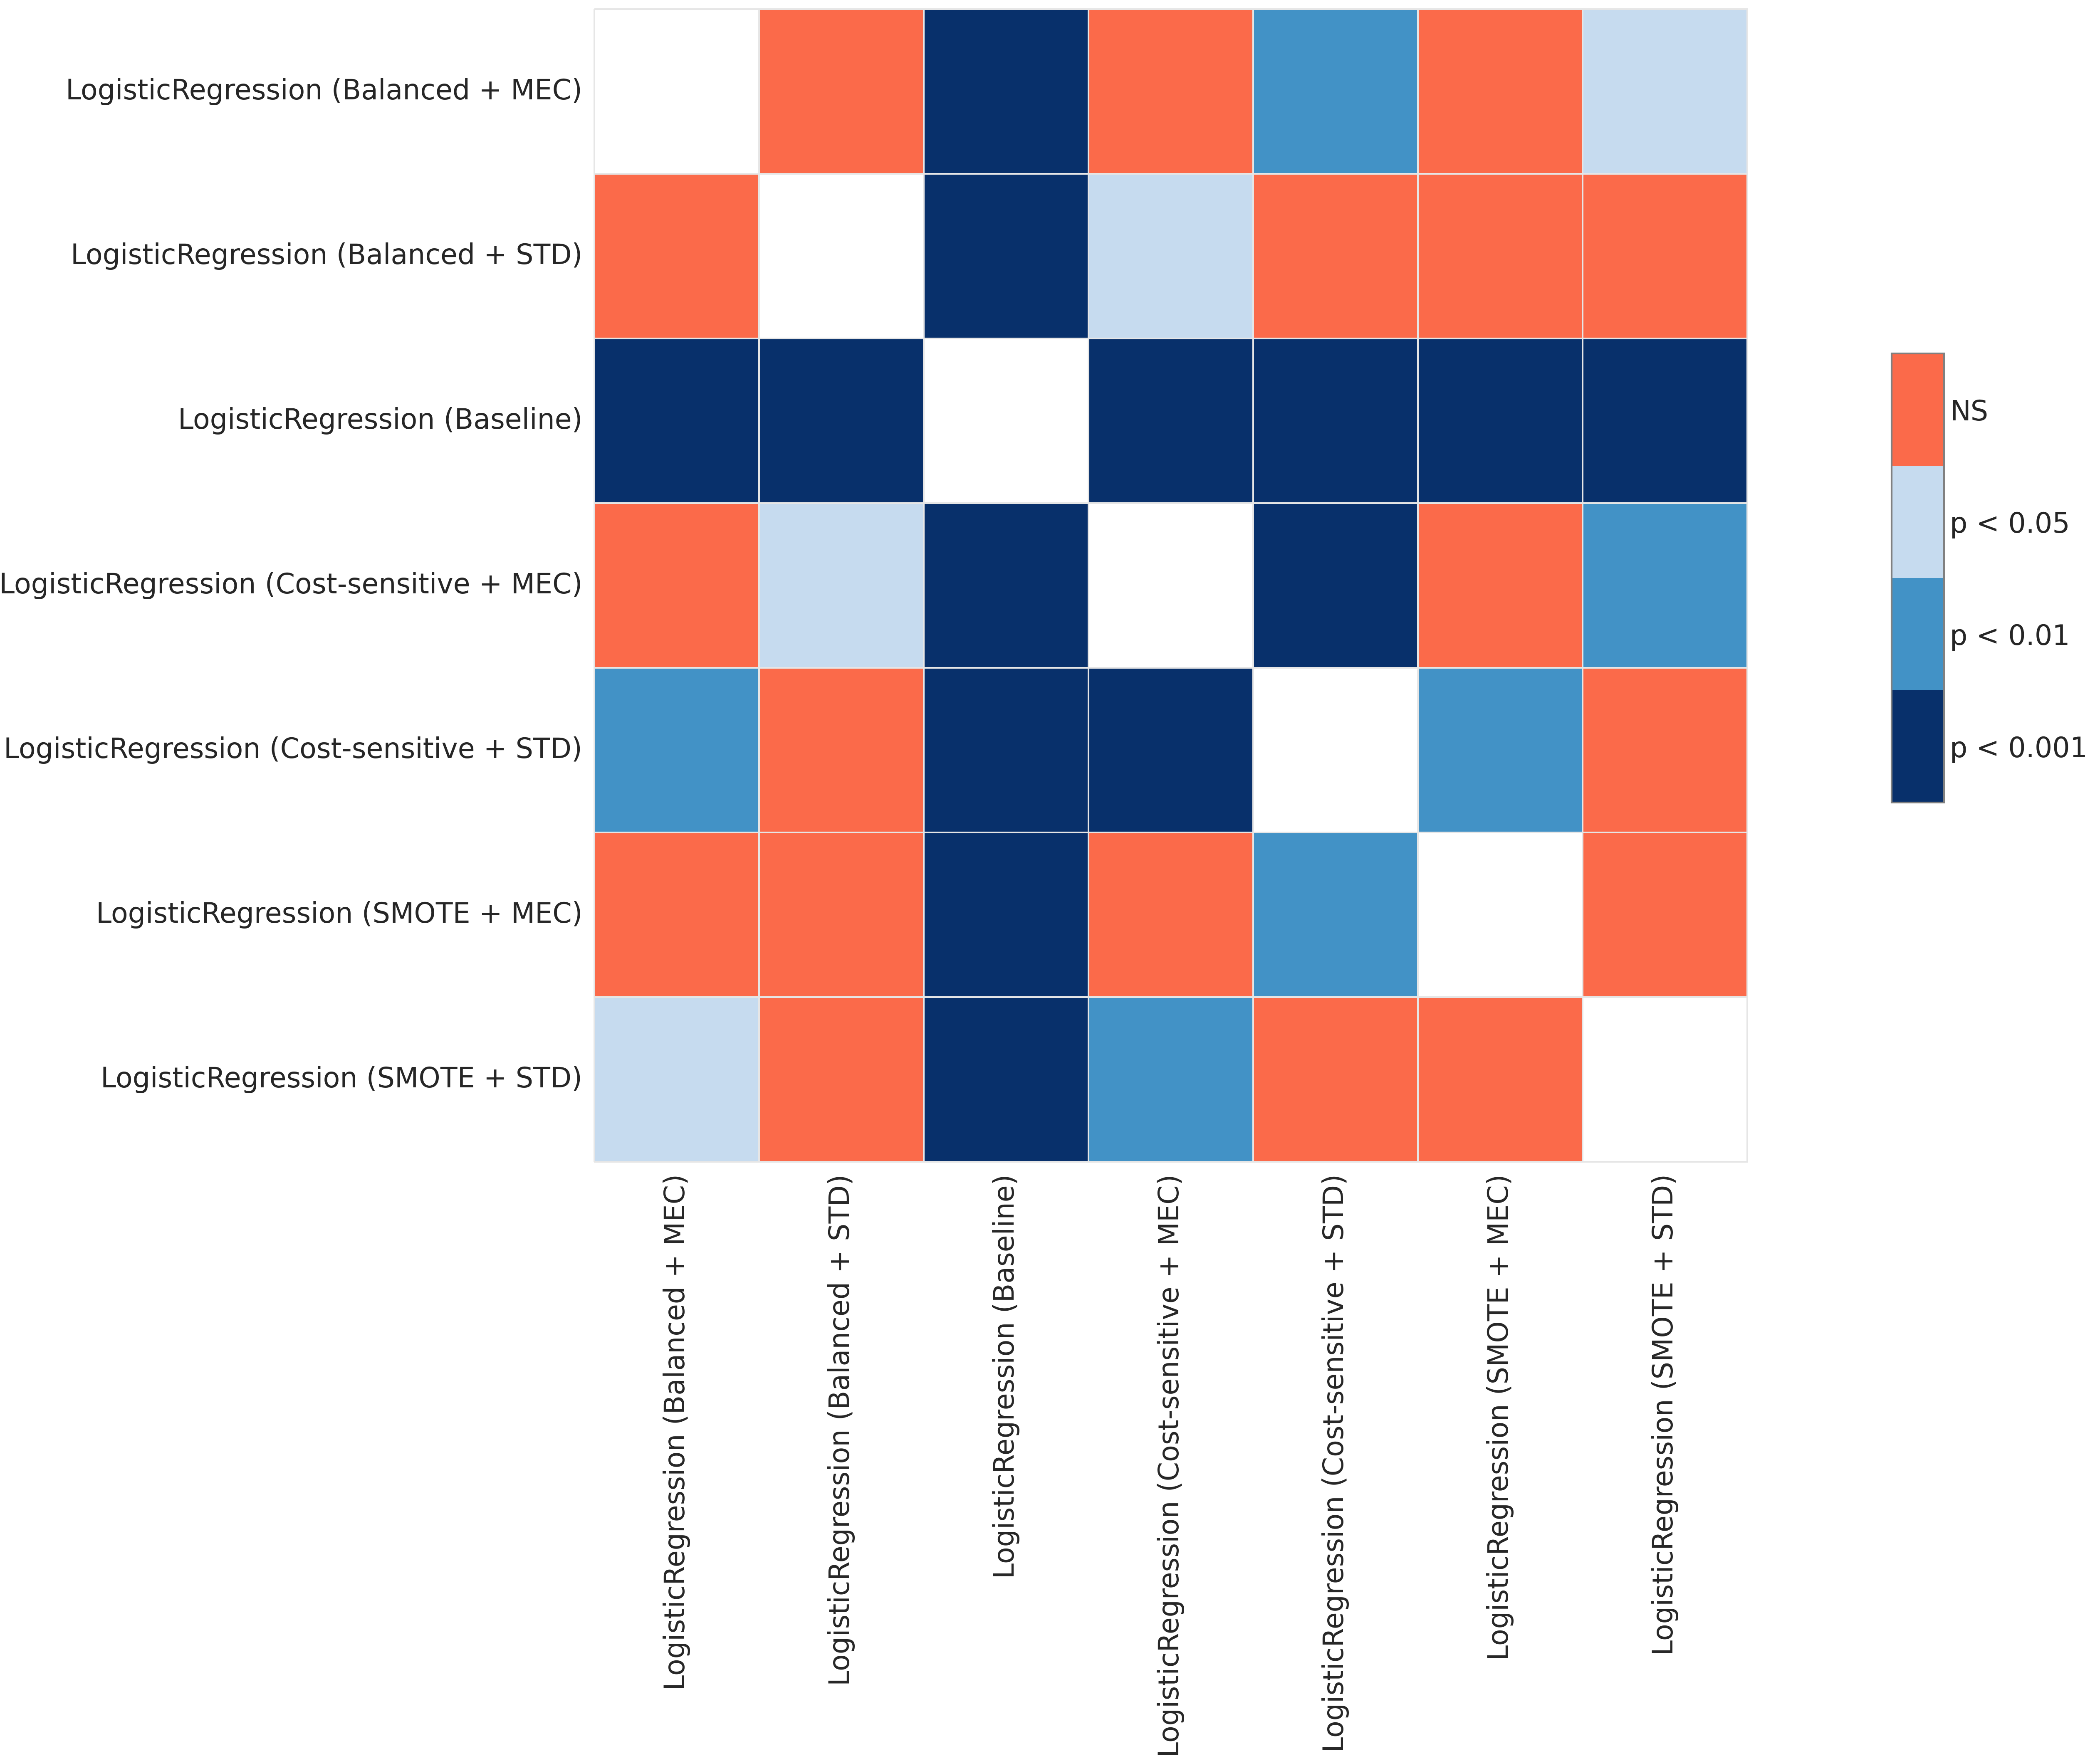
\includegraphics[width=\textwidth, height=0.85\textheight,keepaspectratio]{figures/average_cost_pvalue_heatmap_lr.png}
	\end{center}
\end{frame}

%----------------------------------------------------------------------------------------

\begin{frame}
	\frametitle{Appendix: Static Ensemble Models (p-values matrix)}
	\begin{center}
		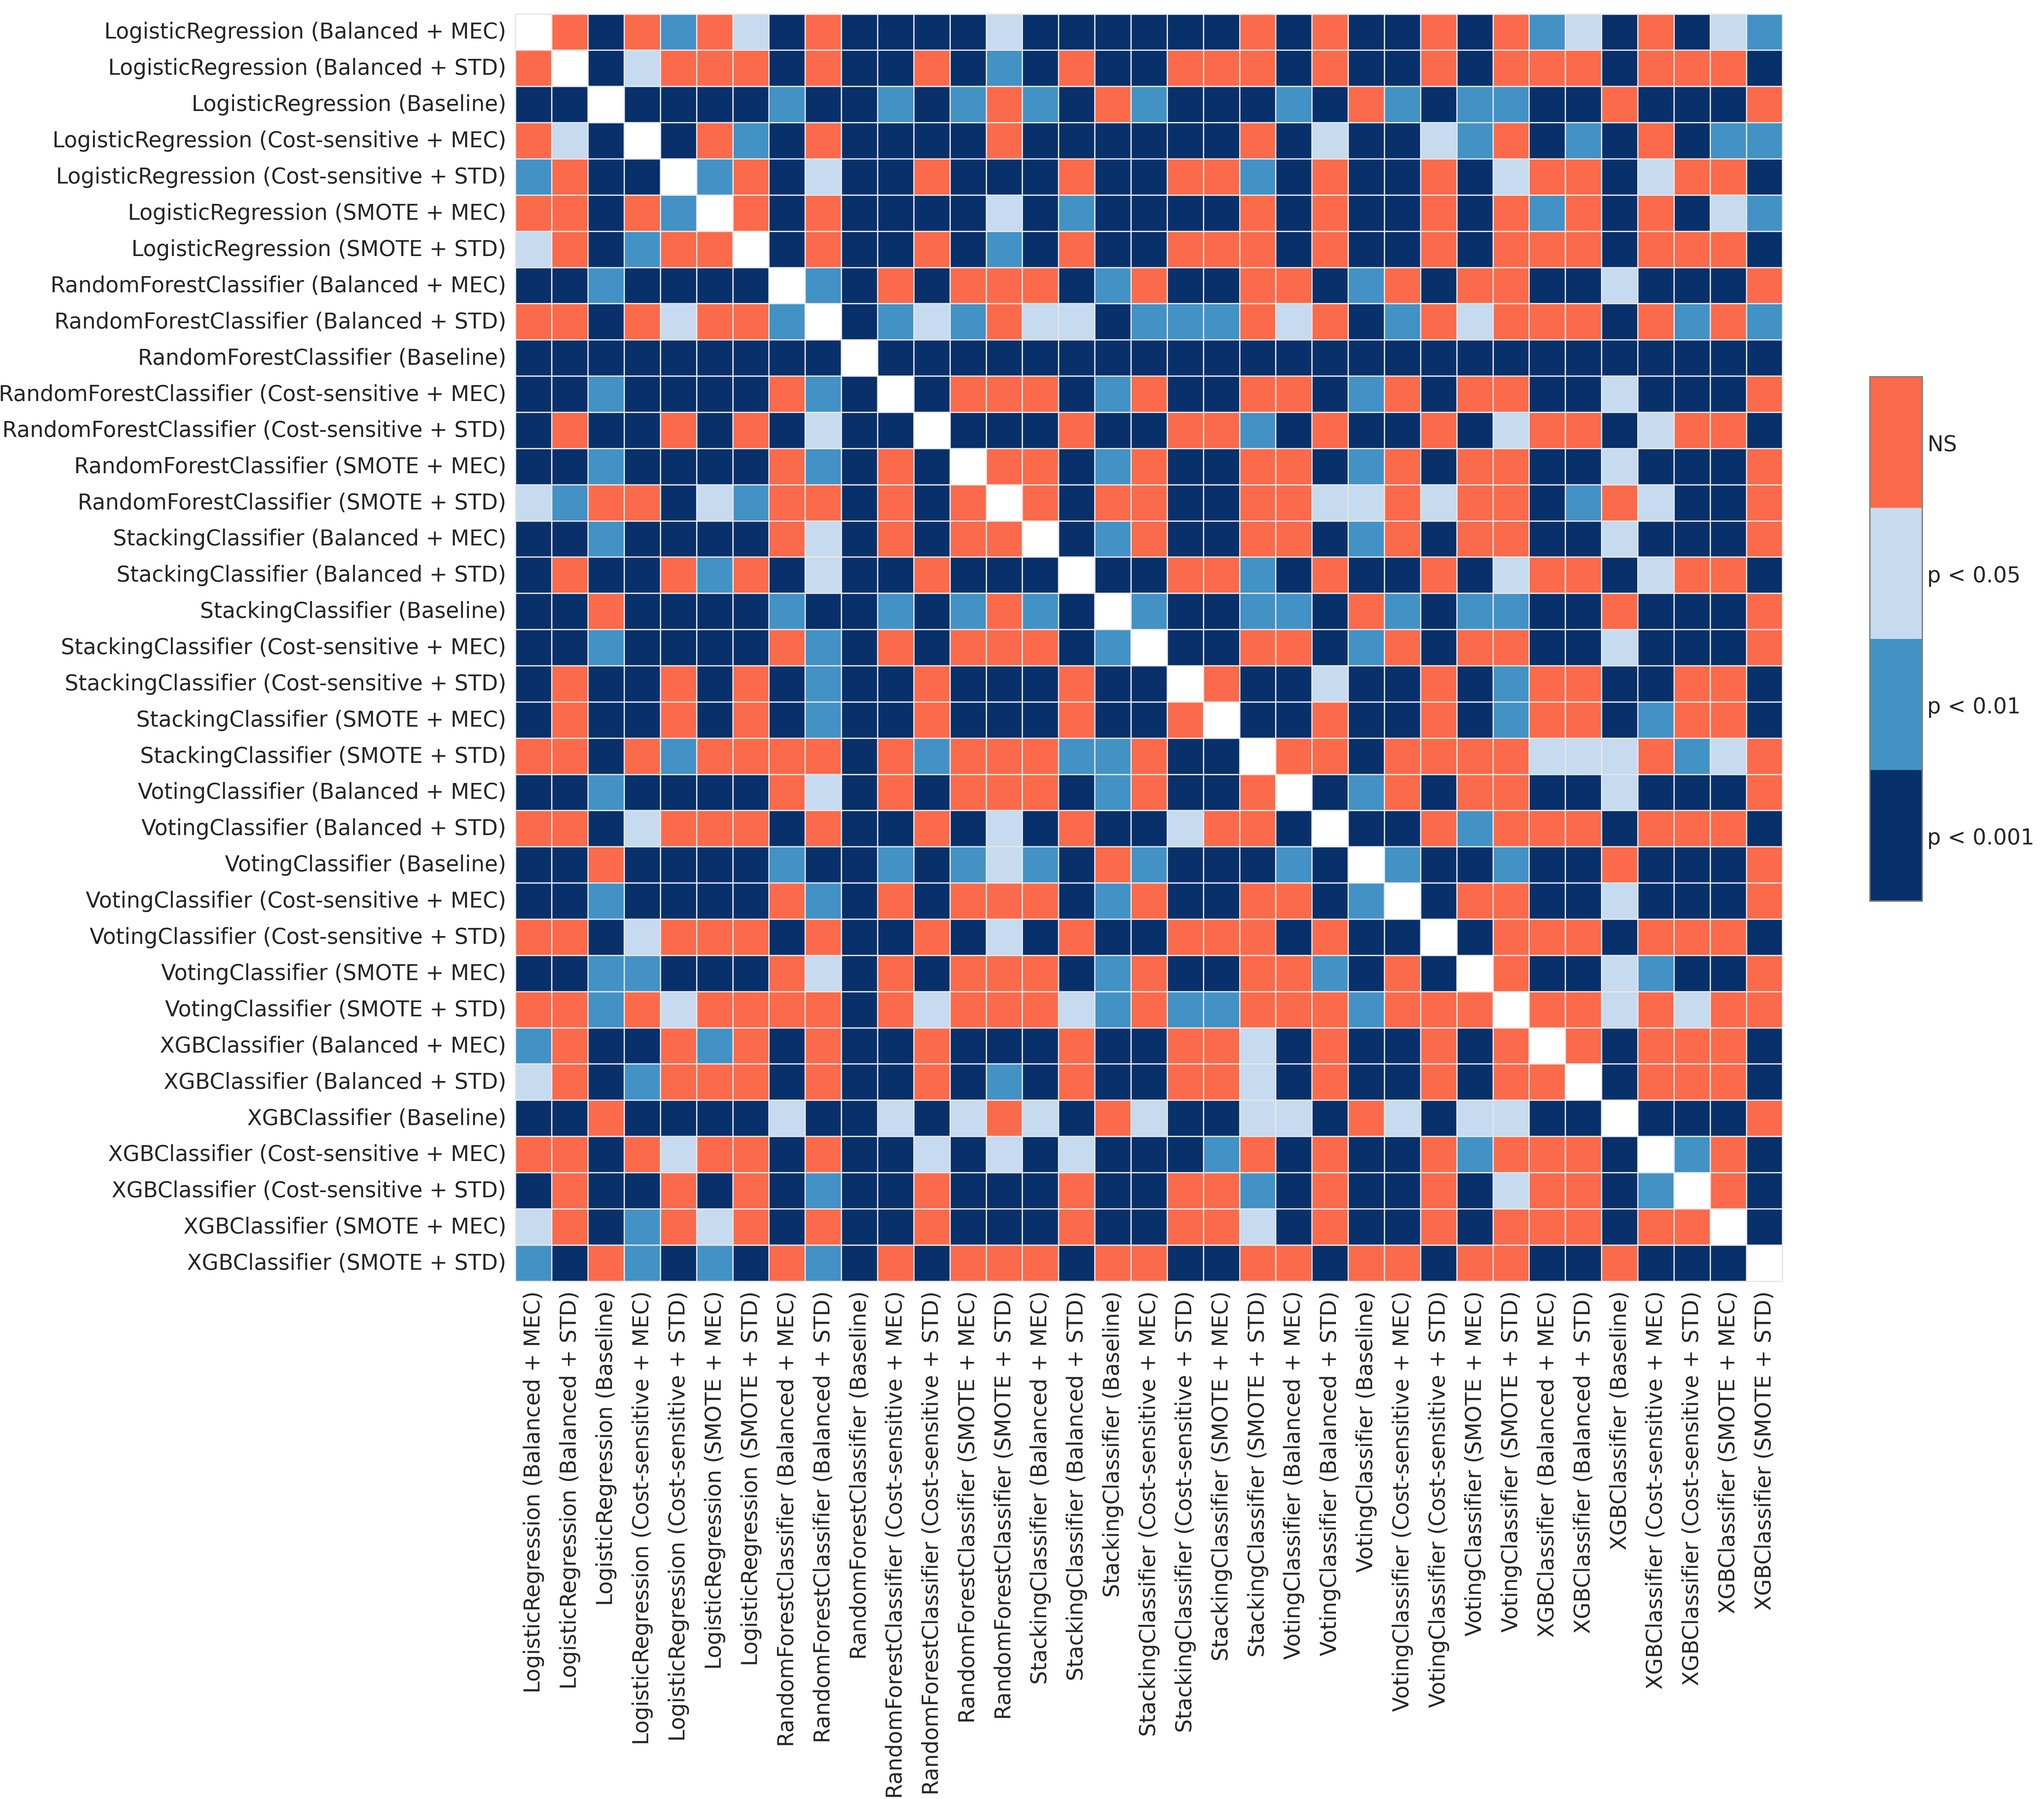
\includegraphics[width=\textwidth, height=0.85\textheight,keepaspectratio]{figures/average_cost_pvalue_heatmap_static.png}
	\end{center}
\end{frame}

%----------------------------------------------------------------------------------------

\begin{frame}
	\frametitle{Appendix: Dynamic Ensemble Models (p-values matrix)}
	\begin{center}
		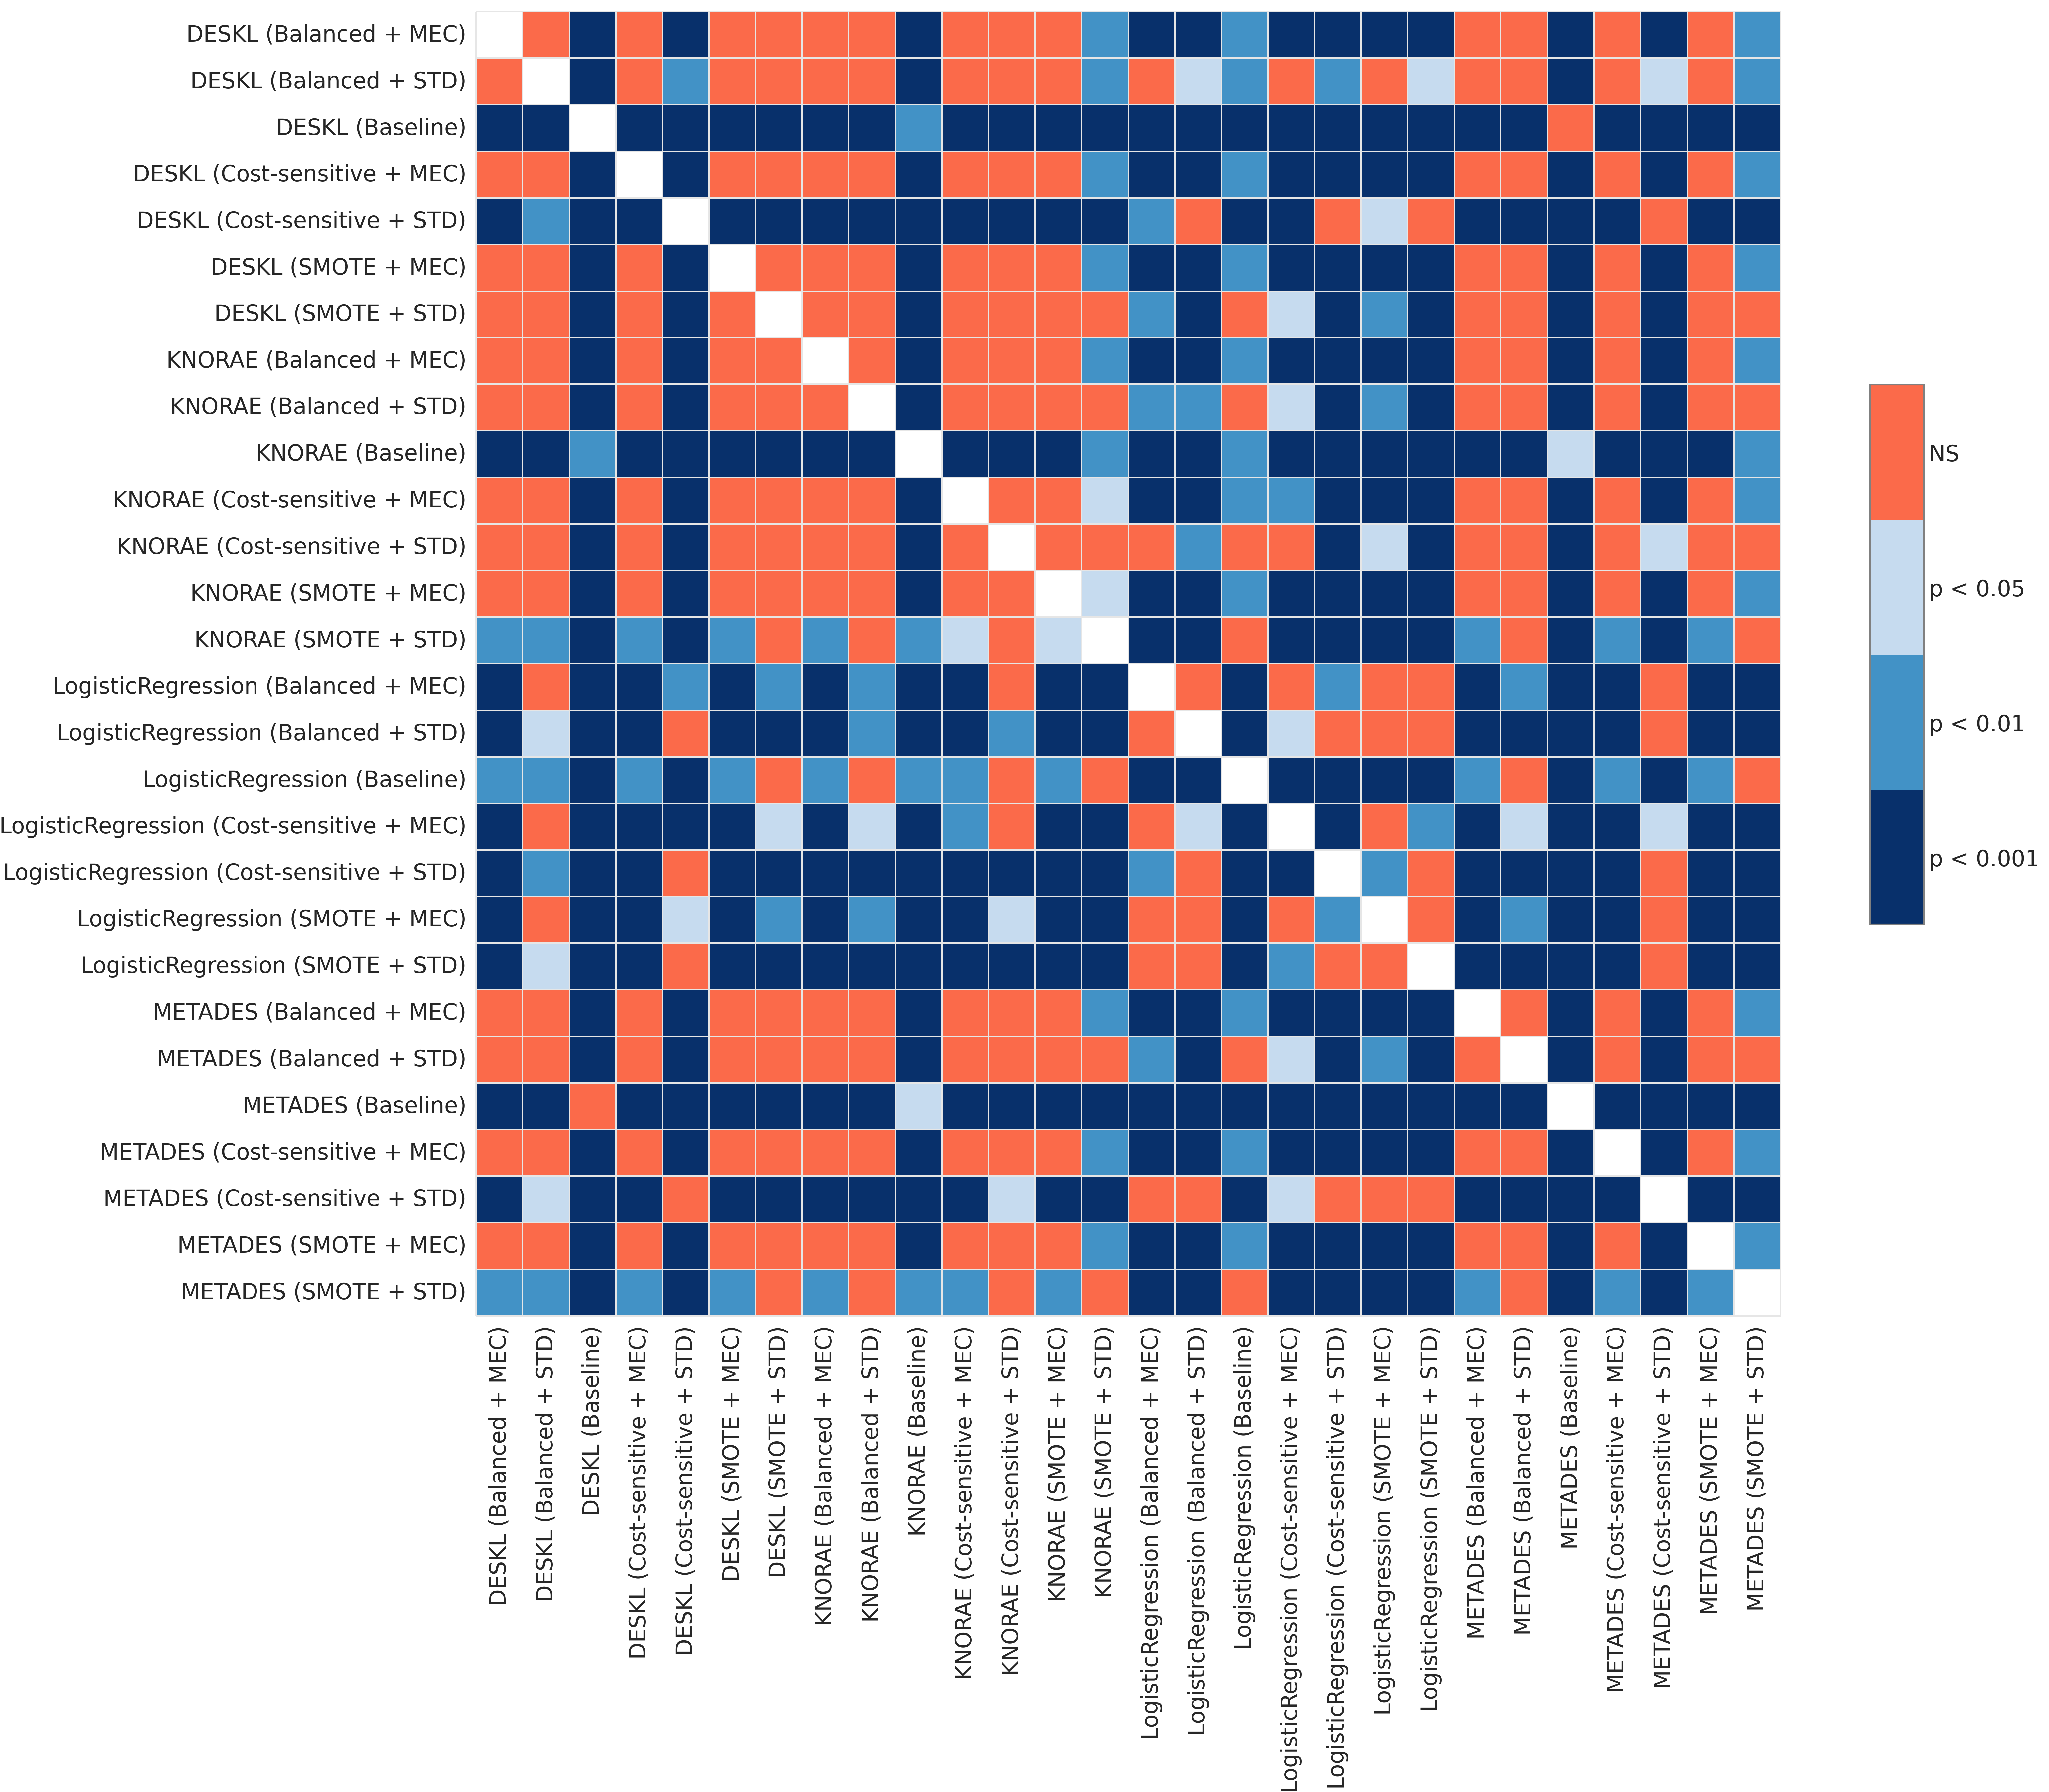
\includegraphics[width=\textwidth, height=0.85\textheight,keepaspectratio]{figures/average_cost_pvalue_heatmap_des.png}
	\end{center}
\end{frame}

%----------------------------------------------------------------------------------------

\begin{frame}
	\frametitle{Appendix: All Models (p-values matrix)}
	\begin{center}
		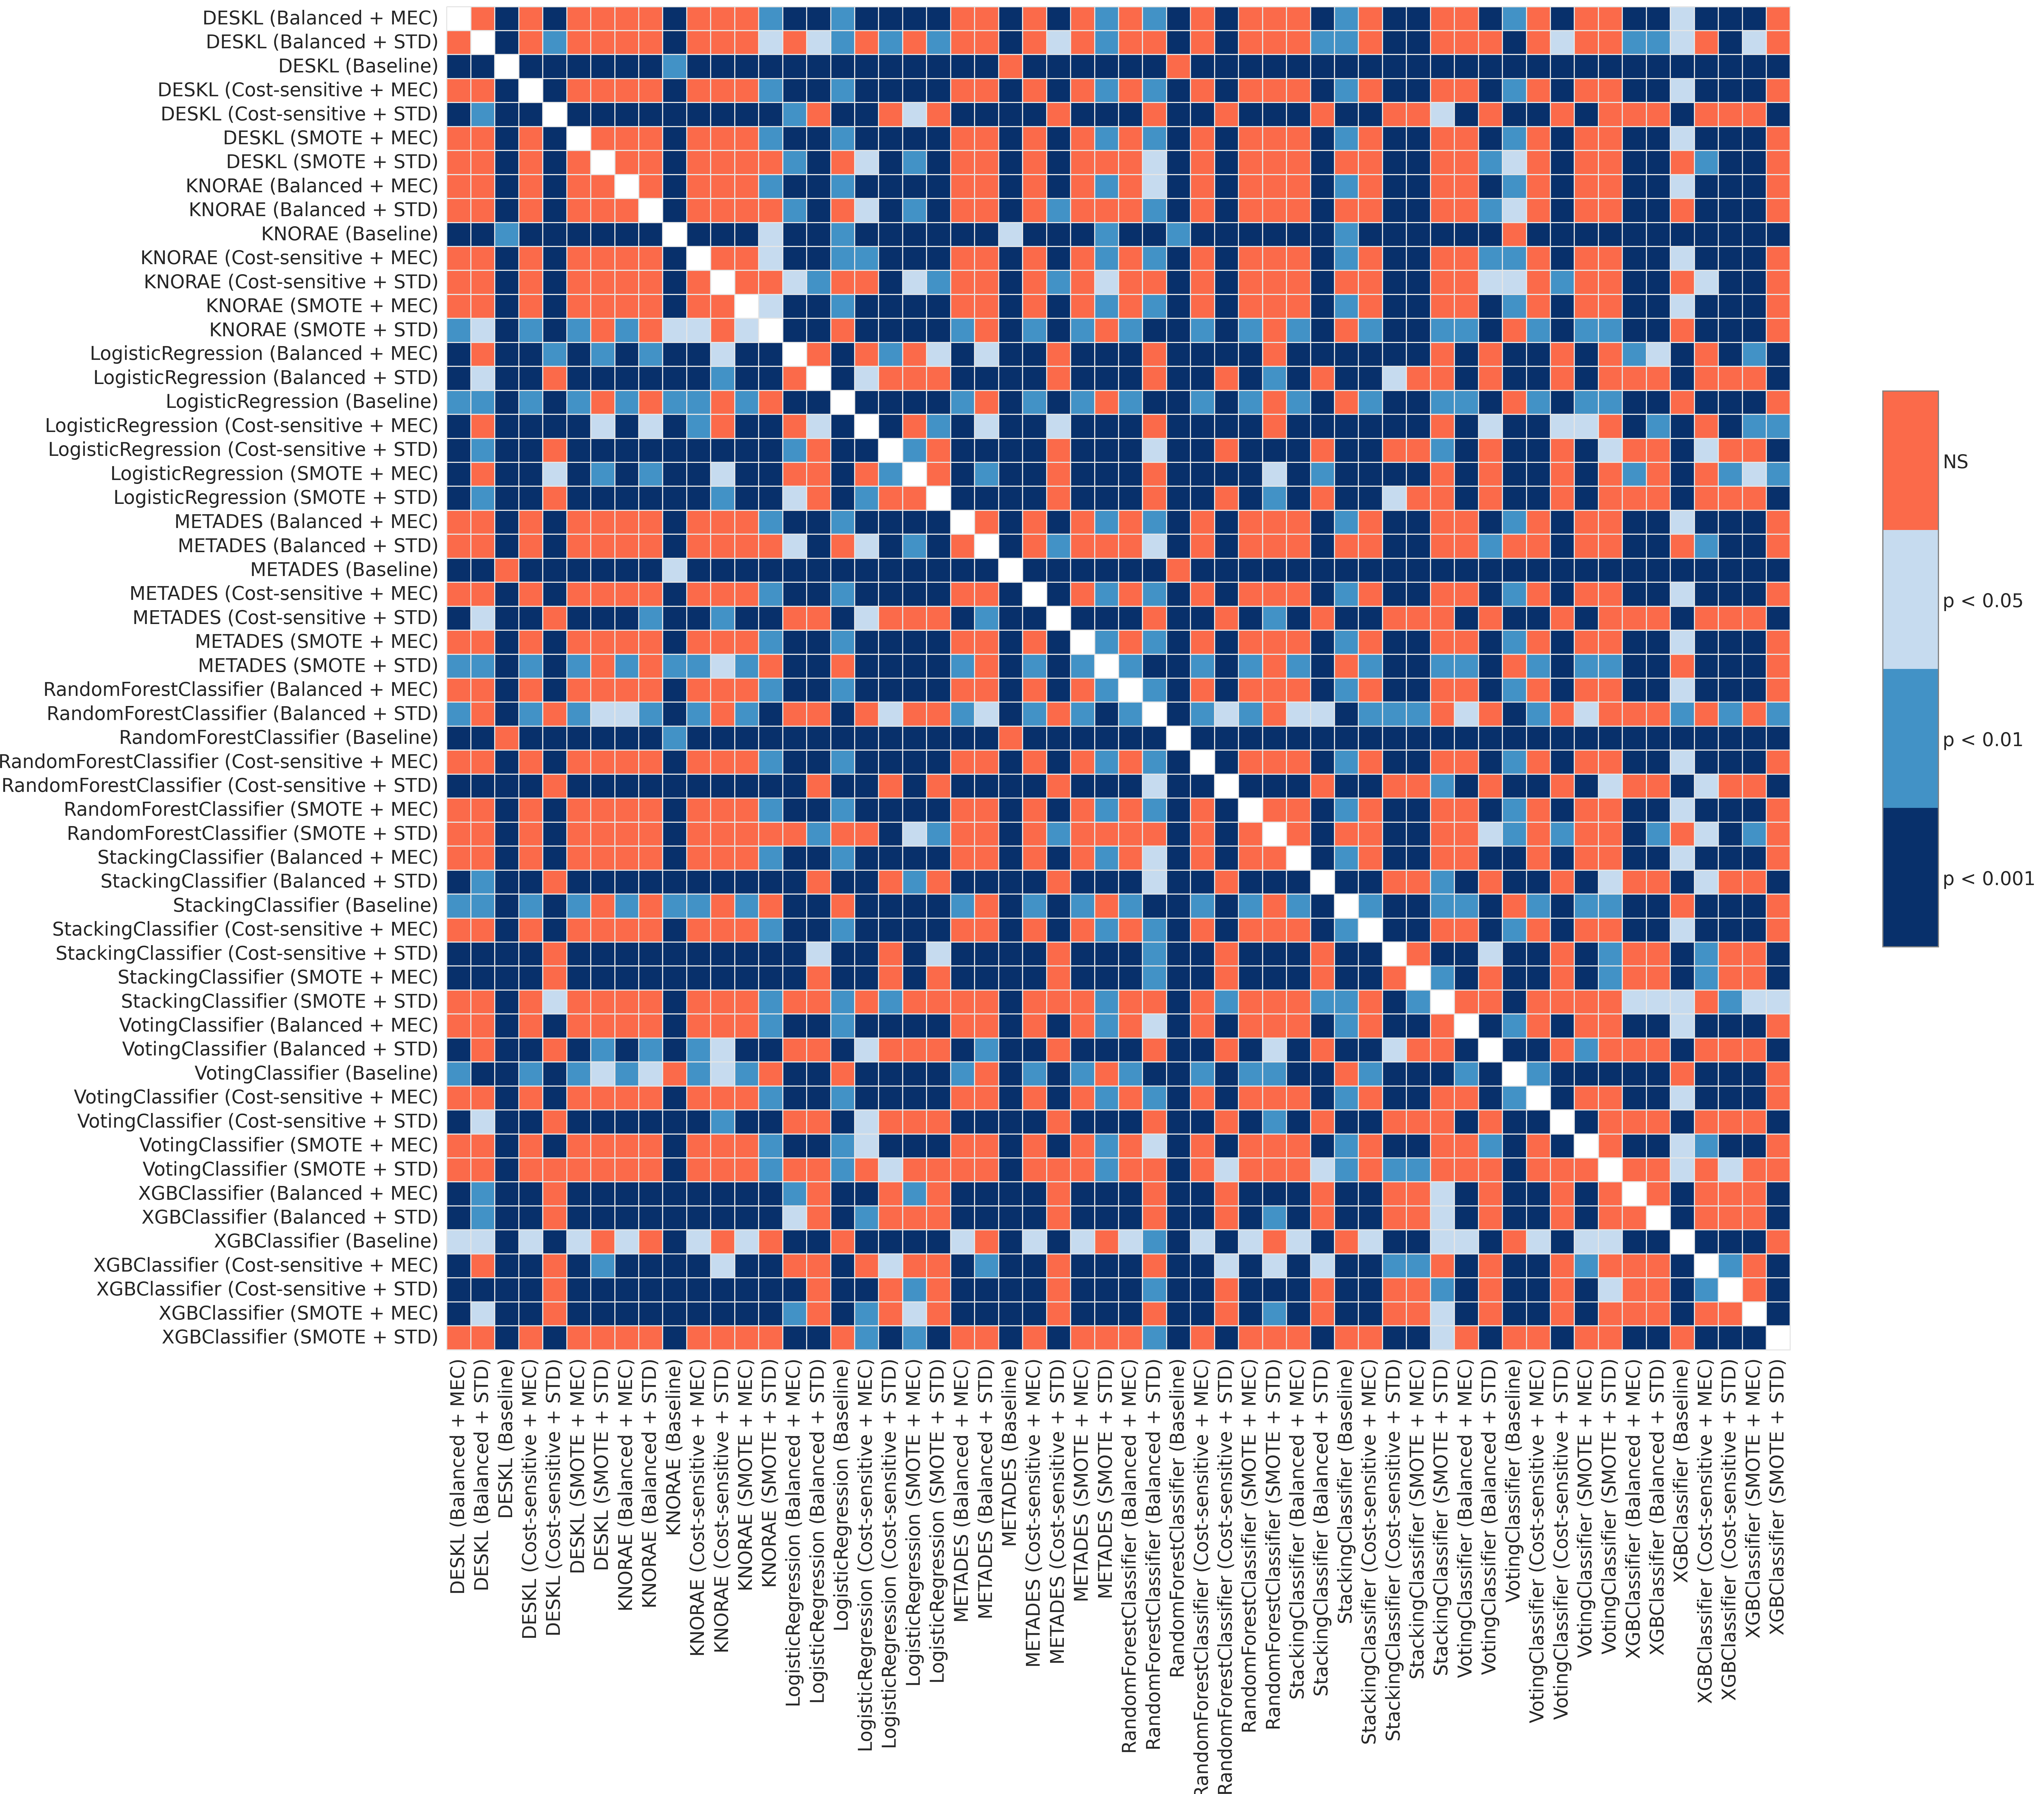
\includegraphics[width=\textwidth, height=0.85\textheight,keepaspectratio]{figures/average_cost_pvalue_heatmap_all.png}
	\end{center}
\end{frame}

%----------------------------------------------------------------------------------------

\end{document}
